\chapter{Metodología de trabajo}
En este capítulo se expone el cuerpo técnico y los procedimientos de ingeniería detallados que permitieron la materialización, puesta en marcha y evaluación del sistema automatizado de cultivo vertical. A través de los apartados siguientes, el lector encontrará la descripción de las etapas analíticas y de diseño conceptual que fundamentaron la selección de las variables operativas y las simulaciones previstas. Asimismo, se detalla el proceso de implementación física del hardware, el cual abarca desde la construcción y optimización de la estructura de los contenedores hasta la selección de los sensores, transductores y actuadores de potencia que conforman la instrumentación electrónica. Finalmente, se documenta el desarrollo de las soluciones mecánicas personalizadas mediante manufactura aditiva, el diseño de la arquitectura del software de control local junto con su integración en plataformas de telemetría en la nube, y la exposición de los resultados experimentales y esquemas de conexión que consolidan la robustez global del prototipo.

\section{Variables de control}
Para dar inicio a la etapa de desarrollo e implementación física del proyecto, resultó indispensable establecer y delimitar las variables físicas y ambientales con mayor representatividad sobre el ciclo biológico de las especies vegetales. El control automatizado de un ecosistema artificial cerrado no puede plantearse de manera genérica; requiere la identificación precisa de aquellos factores que gobiernan la actividad metabólica y el rendimiento fotosintético de los cultivos. Tras un exhaustivo relevamiento de las demandas agronómicas en sistemas de agricultura vertical confinados, se determinó que el control central debía estructurarse en torno a cuatro variables fundamentales: la humedad del sustrato radicular, la intensidad lumínica o iluminancia, la temperatura ambiente y la humedad relativa del aire.

La justificación técnica para la selección y el sensado permanente de cada uno de estos parámetros se detalla a continuación:

En primer lugar, la humedad del sustrato radicular constituye la variable crítica para la supervivencia de la planta, al ser el indicador directo de la disponibilidad hídrica en el suelo. El agua no solo actúa como el vehículo conductor que transporta los nutrientes disueltos desde las raíces hasta las hojas, sino que es un reactivo químico esencial en la fase luminosa de la fotosíntesis. El monitoreo de este parámetro se justifica desde la ingeniería de control como la variable de realimentación principal para el accionamiento de las electroválvulas y la bomba de agua. Mantener esta variable en un rango óptimo previene dos escenarios fatales: el estrés hídrico por marchitamiento debido a la escasez de agua, y la anoxia radicular por exceso de riego, condición donde la saturación de los poros del suelo desplaza al oxígeno, provocando la asfixia y posterior podredumbre de las raíces.

En segundo lugar, la intensidad lumínica o iluminancia es el parámetro motor de todo el sistema de producción vegetal. La luz aporta la energía electromagnética en forma de fotones que las moléculas de clorofila absorben para iniciar la conversión de materia inorgánica en carbohidratos. El sensado de la iluminancia ambiental permite al sistema auditar el funcionamiento real de las luminarias artificiales de espectro completo y cuantificar el aporte lumínico que reciben las plantas. Esta medición justifica la regulación de la variable cronológica del fotoperíodo, asegurando que los cultivos completen las horas de luz necesarias para sus fases vegetativas y de floración, evitando la etiolación, que es el crecimiento debilitado y alargado del tallo cuando la energía lumínica es insuficiente.

En tercer lugar, la temperatura ambiente ejerce un control directo sobre la velocidad de las reacciones bioquímicas y enzimáticas de los vegetales. Cada especie posee un rango térmico óptimo donde su metabolismo funciona con la máxima eficiencia. Si la temperatura desciende por debajo de los límites críticos, los procesos celulares se ralentizan, deteniendo el crecimiento; por el contrario, si la temperatura se eleva en exceso, las proteínas celulares corren el riesgo de desnaturalizarse. El registro continuo de esta variable fundamenta el accionamiento de las etapas de ventilación forzada para disipar el calor térmico acumulado, resguardando la integridad del cultivo frente a fluctuaciones térmicas nocivas.

Finalmente, la humedad relativa del ambiente se seleccionó debido a su impacto directo sobre el proceso de transpiración y la regulación estomática de las hojas. Las plantas abren sus estomas para absorber el dióxido de carbono necesario para la fotosíntesis, liberando vapor de agua en el proceso. Si la humedad del aire es extremadamente baja, la planta se ve forzada a cerrar sus estomas para evitar una deshidratación acelerada, lo que detiene inmediatamente la asimilación de carbono y ralentiza su desarrollo. Si la humedad relativa es excesivamente alta, se reduce la transpiración y se genera un microclima propenso a la proliferación de patógenos y hongos foliares. El monitoreo combinado de la temperatura y la humedad ambiente provee al algoritmo de control la información necesaria para gestionar la renovación del aire, asegurando un equilibrio constante entre la respiración de la planta y la estabilidad de su entorno físico.

\section{Diseño estructural y análisis de sistemas integrados} 

\subsection{Prototipo Inicial}
Para la construcción del primer prototipo, destinado a las pruebas preliminares, se optó por utilizar madera reciclada de bajo costo. El ensamblaje se diseñó con el propósito de soportar la luminaria de espectro completo en la parte superior, dejando espacio suficiente en la base para alojar la maceta, tal como se ilustra a continuación:
\begin{figure}[htbp]
    \centering
    \includegraphics[width=0.5\linewidth]{Imagenes/imagen14.png}
    \caption{Construcción del prototipo inicial}
    \Fuente{propia.}
    \label{fig:placeholder}
\end{figure}
Como se puede observar, la estructura presenta un diseño simple que agilizó su armado para la puesta en marcha del sistema, también se dispuso un cartón que rodeara la maceta con el fin de evitar la dispersión de luz fuera del espacio de la maceta. Esta disposición abierta resultó ventajosa para la integración del hardware, ya que facilitó la instalación del cableado, la conexión de los sensores y facilitar regular la altura del foco. Asimismo, el diseño favoreció la aireación de la planta, contribuyendo a la reducción de la humedad y a una mejor disipación del calor térmico generado.
Durante la fase experimental, se realizaron pruebas preliminares y validaciones técnicas que permitieron identificar oportunidades de optimización en el diseño original. A partir de los datos recolectados en estas iteraciones, se aplicaron ajustes correctivos para maximizar la eficiencia operativa del sistema. Una vez validados los criterios de funcionamiento bajo los estándares previstos, se procedió al diseño e implementación del prototipo final, integrando arquitecturas de hardware y software de mayor robustez.

\subsection{Prototipo Final} 
Tras validar la eficacia del sistema inicial, se procedió al diseño del prototipo definitivo. Este fue proyectado para alojar los cultivos y cumplir con las dimensiones requeridas según las especificaciones del proyecto. Se determinó que las macetas debían poseer una superficie de 0,5m2 cada una; para satisfacer este requerimiento, y considerando las dimensiones de los insumos comerciales disponibles (machimbre, tablones y listones de madera), se optó por una medida estándar de 100cm x 50cm. Se seleccionó madera de pino (Pinus) para la construcción de la estructura debido a su factibilidad económica y a que sus propiedades mecánicas resultan adecuadas para los esfuerzos estructurales previstos en el sistema de cultivo.
Debido a que uno de los objetivos centrales de este trabajo es la optimización de recursos y el aprovechamiento del espacio físico, se implementó una disposición vertical (tipo estantería o rack). Este diseño fue configurado para asegurar la correcta integración de los componentes electrónicos, sensores y actuadores, garantizando la accesibilidad para el mantenimiento y la eficiencia en la distribución del cableado. El diseño final se presenta en la siguiente figura:

\begin{figure}[H]
    \centering
    \begin{minipage}{0.48\textwidth}
        \centering
        \includegraphics[width=\textwidth]{Imagenes/prototipo 2026-04-20 at 11.49.18 AM.png}
    \end{minipage}
    \hfill
    \begin{minipage}{0.48\textwidth}
        \centering
        \includegraphics[width=\textwidth]{Imagenes/prototipo 2026-04-20 at 11.49.25 AM.png}
    \end{minipage}
    \caption{Diseño del prototipo.}
    \Fuente{propia.}
\end{figure}

% Acá podés poner un párrafo de texto

\begin{figure}[H]
    \centering
    \includegraphics[width=0.6\textwidth]{Imagenes/prototipo 2026-04-20 at 11.49.04 AM.png}
    \caption{Vista inferior del prototipo.}
    \Fuente{propia.}
\end{figure}

Una vez establecido el diseño final, se procedió a su construcción física. Durante esta etapa, se presentaron restricciones prácticas que exigieron replantear el montaje original. En primer lugar, la altura total proyectada para el sistema superaba la altura disponible en el laboratorio, lo que hizo obligatorio realizar modificaciones dimensionales. En segundo lugar, se determinó que el peso final de la estructura en conjunto dificultaría considerablemente su traslado y reubicación una vez concluido el proyecto.
Para resolver estos inconvenientes, se rediseñó la estructura adoptando un enfoque modular. El prototipo definitivo quedó conformado por dos módulos de cultivo apilables y desmontables entre sí, acompañados de un tercer módulo totalmente independiente. Esta solución no solo facilitó la logística y el transporte del hardware, sino que también dotó al proyecto de una arquitectura escalable, demostrando empíricamente que el sistema no presenta limitaciones frente a la cantidad de niveles que se deseen integrar.
\begin{figure}[htbp]
    \centering
    \includegraphics[width=0.5\linewidth]{Imagenes/maceta1.jpeg}
    \caption{Implementacion fisica del prototipo}
    \Fuente{propia.}
    \label{fig:placeholder1}
\end{figure}

\begin{figure}[H]
    \centering
    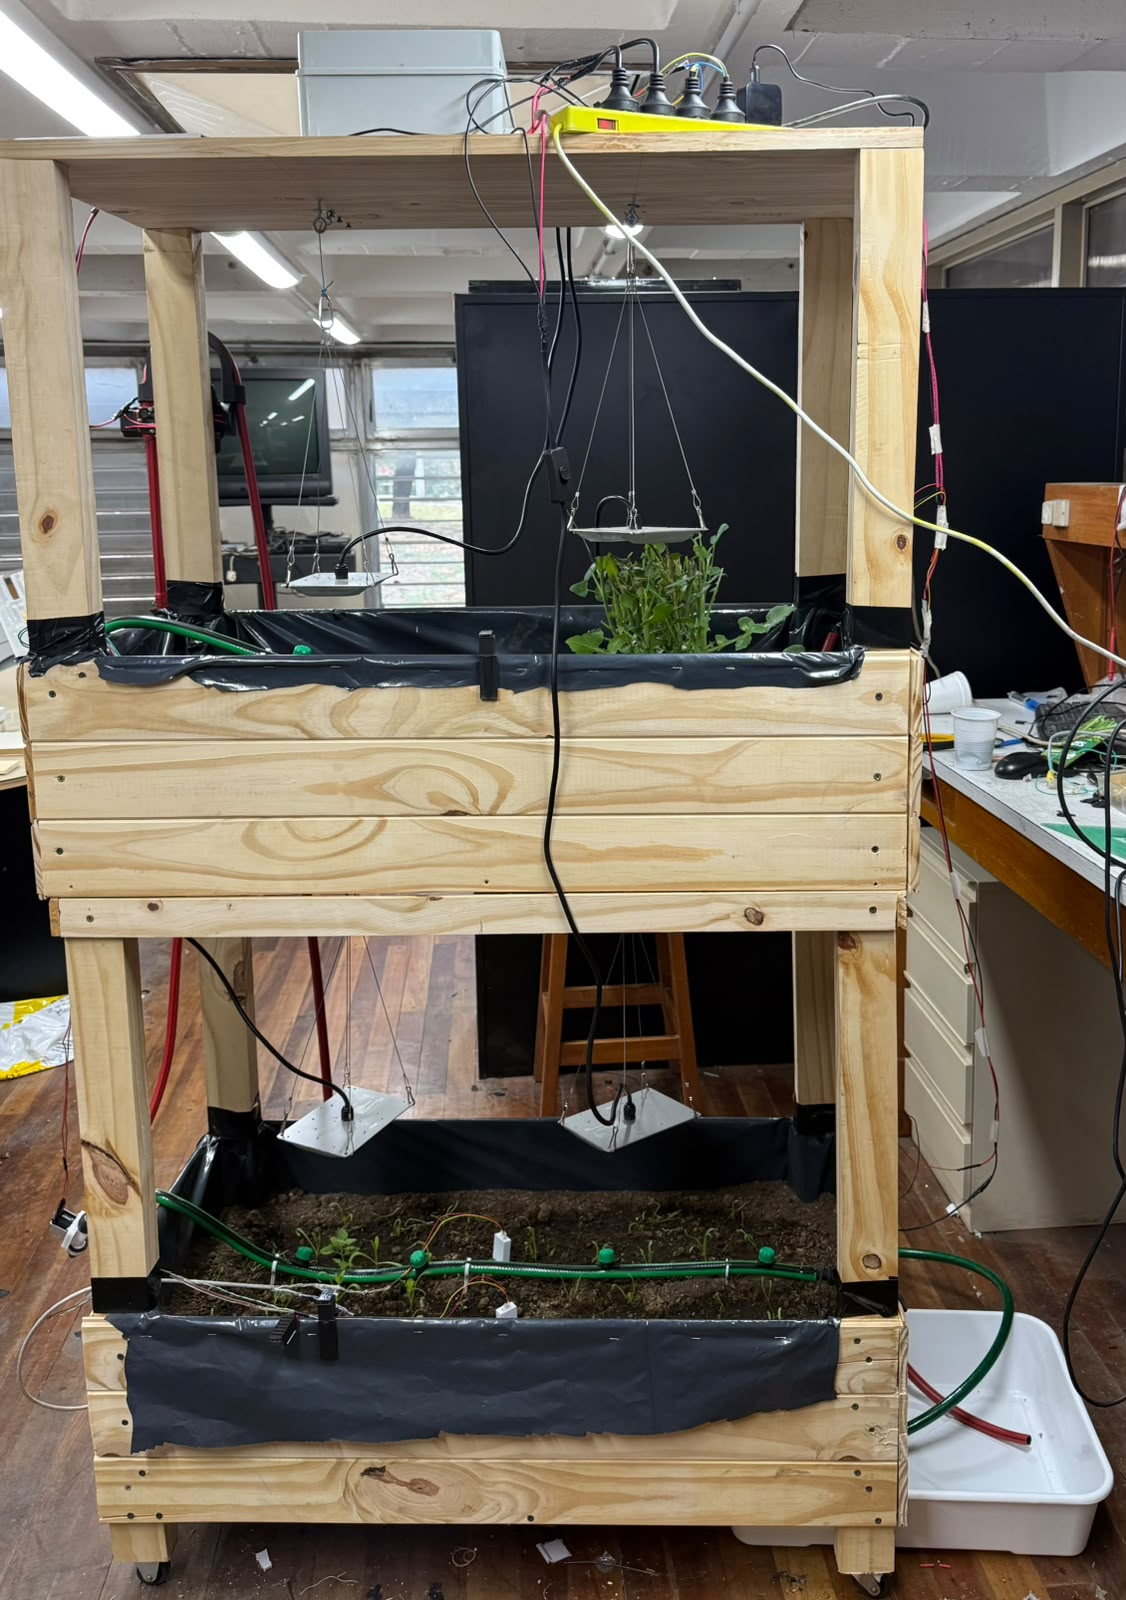
\includegraphics[height=10cm, width=\textwidth, keepaspectratio]{Imagenes/prototipofinal.jpeg}
    \caption{Prototipo en su etapa final.}
    \Fuente{propia.}
\end{figure}

\subsubsection{Impermeabilizacion y drenaje} 
Para prevenir la absorción de humedad por parte de la estructura de madera (condición que podría derivar en hinchamiento, deformación mecánica o degradación biológica), resultó indispensable implementar una barrera física entre el sustrato de cultivo y el contenedor. Los criterios para la selección del material aislante exigían impermeabilidad total, resistencia mecánica para soportar la carga estática de la tierra húmeda, y una alta durabilidad temporal frente a la degradación.
El material seleccionado para satisfacer estos requerimientos fue la lona plástica de uso agrícola (comercialmente conocida como Poliagro), un material sintético de alta resistencia fabricado a base de polietileno o poliéster con recubrimiento de PVC. Este polímero garantiza una impermeabilidad absoluta, cuenta con tratamiento de protección UV y presenta una elevada resistencia al desgarro. Estas características lo convierten en un estándar para aplicaciones agrícolas e industriales de alta exigencia (tales como el revestimiento de reservorios de agua (tanques australianos) y la protección de maquinaria a la intemperie), asegurando así una prolongada vida útil dentro de las condiciones de humedad propias del sistema de cultivo.

\begin{figure}[H]
    \centering
    \begin{minipage}{0.48\textwidth}
        \centering
        \includegraphics[height=10cm, width=\textwidth, keepaspectratio]{Imagenes/imagen3.jpeg}
    \end{minipage}
    \hfill
    \begin{minipage}{0.48\textwidth}
        \centering
        \includegraphics[height=10cm, width=\textwidth, keepaspectratio]{Imagenes/imagen4.jpeg}
    \end{minipage}
    \caption{Proceso de impermeabilización }
    \Fuente{propia.}
\end{figure}

Una vez definida la impermeabilización del contenedor, se procedió al diseño del sistema de drenaje. Este componente representó un desafío técnico significativo debido a las propiedades físico-químicas del poliagro, el cual posee una tensión superficial baja (aproximadamente entre 30 y 31 dinas/cm). Esta baja energía superficial dificulta la humectación y la adhesión de selladores convencionales, complicando la estanqueidad del sistema. El objetivo del diseño era garantizar la evacuación del excedente hídrico para prevenir la anoxia radicular (podredumbre de las raíces), conduciendo el fluido hacia un depósito central de desagüe.
Para la primera iteración, se realizaron seis perforaciones en la base de la maceta, donde se instalaron piezas filtrantes fabricadas en impresión 3D. Estas piezas tenían la función de actuar como filtros de sedimentos para evitar la pérdida de sustrato. Sin embargo, este primer diseño presentó filtraciones considerables; a pesar de haber reforzado las uniones con cinta adhesiva de alta resistencia y selladores elastoméricos, los resultados fueron insatisfactorios, lo que llevó a descartar esta configuración de inmediato.

\begin{figure}[H]
    \centering
    \begin{minipage}{0.48\textwidth}
        \centering
        \includegraphics[height=10cm, width=\textwidth, keepaspectratio]{Imagenes/imagen6.jpeg}
    \end{minipage}
    \hfill
    \begin{minipage}{0.48\textwidth}
        \centering
        \includegraphics[height=10cm, width=\textwidth, keepaspectratio]{Imagenes/imagen7.jpeg}
    \end{minipage}
    \caption{Configuración del desagüe.}
    \Fuente{propia.}
\end{figure}

En una segunda fase, se diseñaron nuevos dispositivos de drenaje mediante manufactura aditiva, incorporando un sistema de acoplamiento roscado. El propósito de la rosca era ejercer una presión mecánica uniforme contra la estructura de madera para minimizar los espacios intersticiales. No obstante, persistieron fugas en la interfaz entre el poliagro y la madera. Tras una serie de ensayos experimentales, se determinó que la solución más efectiva consistía en la integración de dos juntas de estanqueidad (arandelas de goma sellantes) dispuestas en ambos puntos de contacto. Esta configuración final permitió alcanzar una estanqueidad total, eliminando el goteo y asegurando la integridad del sistema de drenaje.

\begin{figure}[H]
    \centering
    \begin{minipage}{0.48\textwidth}
        \centering
        \includegraphics[height=10cm, width=\textwidth, keepaspectratio]{Imagenes/imagen16.jpeg}
    \end{minipage}
    \hfill
    \begin{minipage}{0.48\textwidth}
        \centering
        \includegraphics[height=10cm, width=\textwidth, keepaspectratio]{Imagenes/imagen17.jpeg}
    \end{minipage}
    \caption{Conducto de desagüe impreso en 3D.}
    \Fuente{propia.}
\end{figure}

Una vez establecido el sistema de drenaje en la base de los contenedores, se procedió a diseñar la red de conducción para dirigir el agua hacia el depósito colector. Dado que cada módulo cuenta con seis puntos de desagüe, fue necesario planificar el tendido de las líneas de transporte desde las piezas filtrantes impresas en 3D hasta el destino final.
En esta etapa, el diseño exigió una rigurosa optimización de la disposición espacial. Por un lado, las líneas de conducción requerían un gradiente de inclinación (pendiente mínima) constante para asegurar el flujo del agua por gravedad, evitando así el estancamiento dentro del circuito. Por otro lado, la naturaleza compacta de la estructura vertical obligaba a aprovechar al máximo el reducido volumen disponible debajo de los cultivos.
Con el objetivo de minimizar la cantidad de insumos requeridos (metros de manguera) y lograr un enrutamiento ordenado, se diseñaron y fabricaron mediante manufactura aditiva racores de derivación tipo "Y". Estos acoples a medida permitieron consolidar múltiples líneas de drenaje en conductos principales de forma eficiente, resolviendo las restricciones de espacio. La configuración final del sistema de conducción se ilustra a continuación:

\begin{figure}[H]
    \centering
    \includegraphics[height=10cm, width=\textwidth, keepaspectratio]{Imagenes/desague1.jpeg}
    \caption{Instalacion de desagüe.}
    \Fuente{propia.}
\end{figure}

\subsubsection{Arquitectura mecánica modular y acoplamiento estructural}
Con el propósito de optimizar la portabilidad y simplificar las tareas de mantenimiento, se proyectó un sistema de desacoplamiento estructural en los contenedores de cultivo. Cada módulo posee la capacidad de separarse de la sección inmediatamente inferior mediante uniones por encastre geométrico, una solución de diseño que confiere una elevada estabilidad estática ante las cargas nominales del sustrato y, simultáneamente, agiliza los procedimientos de desarmado. Asimismo, el módulo posicionado en el estrato superior incorpora ruedas que facilitan el desplazamiento independiente de la estructura dentro del espacio de laboratorio.
imagen 

\section{Unidad Central de Procesamiento: Raspberry Pi 4 Model B}
La selección de la unidad de procesamiento central constituyó una decisión estratégica orientada a garantizar la modularidad, la robustez informática y la proyección a largo plazo del sistema. En lugar de optar por microcontroladores tradicionales de arquitectura básica (como las familias ATmega o los módulos ESP), se seleccionó la computadora de placa única (\textit{Single Board Computer} o SBC) Raspberry Pi 4. Esta determinación se fundamentó en la previsión de un crecimiento modular del sistema, el cual contempla la adición de múltiples módulos de cultivo y macetas automatizadas sin un límite predefinido, asegurando que la capacidad de cómputo y el procesamiento de datos concurrentes no representen un cuello de botella tecnológico.

Frente a los microcontroladores estándar del mercado, la Raspberry Pi 4b presenta ventajas técnico-operativas disruptivas. En primer lugar, su procesador ARM Cortex-A72 de cuatro núcleos a $1{,}5\text{ GHz}$ ofrece una potencia de cálculo aritmético-lógico exponencialmente superior. En segundo lugar, al operar bajo un sistema operativo multitarea completo basado en Linux, el dispositivo permite la ejecución de hilos en paralelo (\textit{multithreading}), la gestión nativa de bases de datos relacionales o no relacionales en el almacenamiento local, y el despliegue de servidores web concurrentes para interfaces de usuario avanzadas; tareas que saturarían la memoria de un microcontrolador. Asimismo, la presencia de conectividad de red avanzada por hardware, como el puerto Gigabit Ethernet y los módulos integrados de Wi-Fi de doble banda y Bluetooth 5.0, optimizan la interoperabilidad y la transmisión de datos a sistemas remotos.

Se reconoce que, en la etapa actual de desarrollo del prototipo, no se está explotando al máximo la capacidad nominal de procesamiento de este dispositivo. No obstante, este sobredimensionamiento controlado constituye un criterio de diseño defensivo y escalable. La integración futura de algoritmos de optimización hídrica o rutinas de visión computacional para el análisis foliar no requerirá una reestructuración del hardware de control. 

Más allá de los límites físicos del presente proyecto, esta elección de hardware traza el inicio del camino hacia el paradigma de las ciudades inteligentes (\textit{Smart Cities}). La arquitectura de software desplegada sobre la Raspberry Pi 4b permite concebir este prototipo no como un elemento aislado, sino como un nodo genérico de una red distribuida. Esta visión de diseño facilita la interconexión e interoperabilidad con otras granjas inteligentes y proyectos de investigación complementarios, permitiendo que futuras tesis puedan tejer una red de monitoreo y producción automatizada a escala urbana, coordinada mediante protocolos robustos de comunicación industrial e Internet de las Cosas (IoT).
\begin{figure}[H]
    \centering
    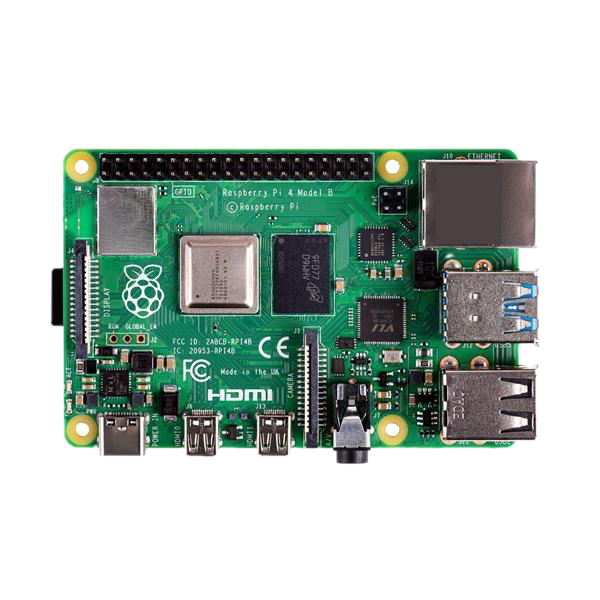
\includegraphics[height=10cm, width=\textwidth, keepaspectratio]{Imagenes/raspberrypi4sf.png}
    \caption{Raspberry Pi 4 Model b.}
    \Fuente{\cite{foto_raspberry_emakers}}
\end{figure}

\section{Selección de componentes}

\subsection{Sustrato}
La selección del sustrato constituyó una fase crítica en el diseño del sistema, ya que el suelo no solo actúa como el soporte físico de las especies vegetales, sino que funciona como la interfaz principal para la absorción de nutrientes y el intercambio gaseoso radicular. Asimismo, las propiedades físicas del sustrato están intrínsecamente ligadas al desempeño del sistema de drenaje diseñado: una elección incorrecta podría derivar en la compactación del medio, afectando la conductividad hidráulica y provocando anoxia radicular (asfixia de las raíces por acumulación de agua).
Tras un análisis comparativo de las opciones disponibles en el mercado, se evaluaron variables de costo, densidad, carga nutricional y, fundamentalmente, la capacidad de infiltración. Finalmente, se optó por una mezcla de tierra fértil compuesta por los siguientes elementos, cada uno cumpliendo una función técnica específica dentro del ecosistema del prototipo:

\textbf{Tierra negra y Compost orgánico:} Constituyen la base nutricional del sustrato. El compost aporta materia orgánica descompuesta y microorganismos beneficiosos que facilitan la disponibilidad de nitrógeno, fósforo y potasio, esenciales para el crecimiento vegetativo.

\textbf{Perlita (Silicato de aluminio):} Este componente mineral es vital para la ingeniería del suelo en cultivos confinados. Debido a su estructura porosa y baja densidad, evita la compactación del sustrato, asegurando una aireación óptima de las raíces y facilitando un drenaje rápido que previene la saturación hídrica.

\textbf{Resaca de río:} Aporta una textura ligera y fibrosa que mejora la estructura del suelo. Su función principal es equilibrar la retención de humedad sin sacrificar la porosidad, permitiendo que el agua se distribuya de manera uniforme antes de ser evacuada por el sistema de drenaje.

\textbf{Pinocha (Acículas de pino):} Su incorporación cumple un rol doble; por un lado, ayuda a mantener un pH ligeramente ácido (ideal para la mayoría de los cultivos de huerta vertical) y, por otro, mejora la estructura mecánica del suelo, evitando que se apelmace con el paso del tiempo y las sucesivas sesiones de riego.

Esta combinación sinérgica garantizó un entorno de crecimiento estable, permitiendo que el hardware de monitoreo (sensores de humedad) registre valores consistentes y que el sistema de drenaje opere según las especificaciones de diseño, asegurando una evolución saludable de los cultivos a lo largo de las pruebas.

\subsection{Sensores y conversor}

\subsubsection{Sensor de humedad ambiente y temperatura}
Para controlar estas variables, se utilizó un sensor digital DHT22 \cite{aosong_dht22}. Esta elección se justifica por su rango completo de medición de humedad relativa (0 a 100), el cual supera las limitaciones del DHT11 (20 a 90). Asimismo, ofrece una resolución y estabilidad decimal críticas para lograr un control preciso de los parámetros del sistema. Desde la perspectiva del hardware, destaca por su simplicidad analógica al prescindir de un conversor analógico-digital (ADC), comunicándose mediante un protocolo de un único hilo conectado directamente a los pines GPIO del microcontrolador. Finalmente, el componente fue seleccionado por su bajo costo y su amplia disponibilidad en el mercado.
\begin{figure}[H]
    \centering
    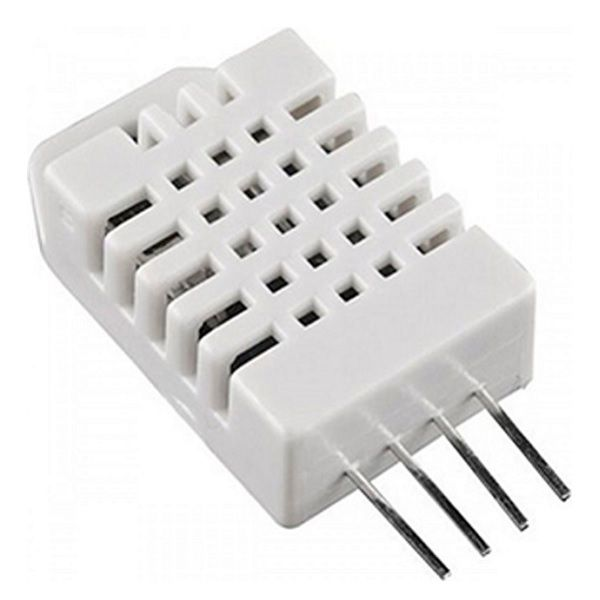
\includegraphics[height=10cm, width=\textwidth, keepaspectratio]{Imagenes/dht22.jpeg}
    \caption{SensorDHT22.}
    \Fuente{\cite{foto_sensor_dht22}}
\end{figure}

\subsubsection{Sensor de iluminancia}
Para la cuantificación de la intensidad lumínica ambiental se seleccionó el sensor digital BH1750 \cite{sensor_iluminancia} en lugar de transductores analógicos resistivos (LDR). Esta decisión se fundamenta en su capacidad para entregar lecturas directas en unidades de lux (lx) con una respuesta espectral calibrada de fábrica que permite distinguir longitudes de onda desde los 400nm hasta 700nm convirtiendose en un candidato ideal para realizar las mediciones para los cultivos. Al integrar un conversor analógico-digital de 16 bits y acondicionamiento de señal interno, el dispositivo ofrece un amplio rango dinámico (de $1\ lx$ a $65535\ lx$) con resolución decimal, garantizando la linealidad de los datos sin saturación ni necesidad de algoritmos de calibración complejos. Asimismo, su interfaz de comunicación basada en el protocolo I2C optimiza el uso de los recursos de hardware del microcontrolador al requerir únicamente dos líneas de datos compartidas. Debido a las caracteristicas anteriores, que cumplen con las especificaciones solicitadas, sumado a su bajo coste, se selecciono este modulo.
\begin{figure}[H]
    \centering
    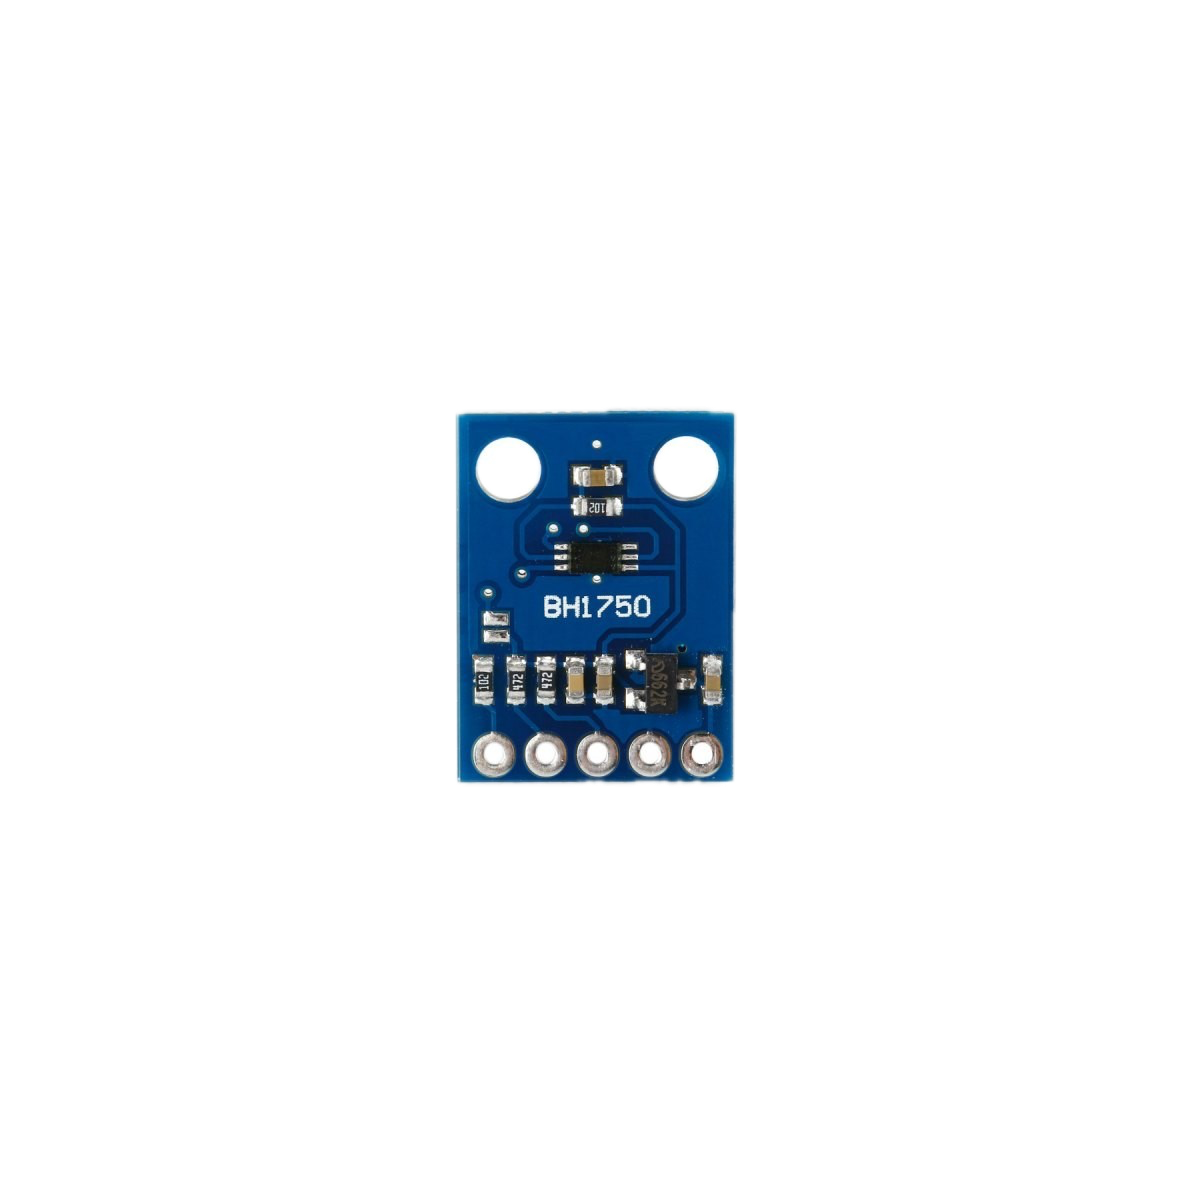
\includegraphics[height=10cm, width=\textwidth, keepaspectratio]{Imagenes/bh1750 Background Removed.png}
    \caption{Sensor bh1750.}
    \Fuente{\cite{foto_sensor_bh1750}}
\end{figure}

\subsubsection{Higrómetro de suelo}
El sensor de humedad de suelo HD-38 \cite{suelo_capacitivo_resistivo} se preseleccionó por su compatibilidad de señal (analógica/digital) y su geometría, cuya longitud de terminales favorecía la medición en la zona radicular profunda. Aunque el fabricante especificaba un tratamiento anticorrosivo para entornos críticos, el desempeño del dispositivo en condiciones operativas reales fue deficiente, exhibiendo una severa pérdida de linealidad y sensibilidad que redujo su funcionamiento a una detección binaria (seco/mojado). Con el objetivo de optimizar su comportamiento, se evaluaron múltiples configuraciones experimentales: control por software del ciclo de trabajo del sensor para mitigar la electrólisis, inserción de un espaciador dieléctrico entre electrodos, variación de la profundidad de enterramiento, recalibración de las etapas del ADC y modificación de las resistencias de acoplamiento. Al no registrarse mejoras significativas en la estabilidad y repetibilidad de las lecturas, se determinó la inviabilidad técnica del componente, procediendo a su descarte definitivo.
Durante la segunda fase de evaluación de higrómetros se implementó un sensor capacitivo \cite{dfrobot_sen0193} donde el esquema de conexion era identico al sensor anterior, pero ahora con el propósito de mitigar la degradación por electrólisis identificada en el dispositivo previo. Debido a su encapsulado y aislamiento galvánico, los electrodos permanecen inmunes a la corrosión, asegurando la estabilidad temporal de las lecturas. El principio de operación se basa en la variación de la capacitancia del entorno, empleando el sustrato como dieléctrico; de este modo, se prescinde del contacto óhmico directo con las sales y el agua, atenuando la deriva en las mediciones y minimizando los requerimientos de recalibración. Tras la puesta en marcha del sistema, se verificó un incremento significativo en la linealidad y repetibilidad de los datos en todo el espectro físico (desde la condición de sequedad extrema hasta la saturación hídrica), proporcionando la precisión requerida para el ajuste y optimizacion del riego.
\begin{figure}[H]
    \centering
    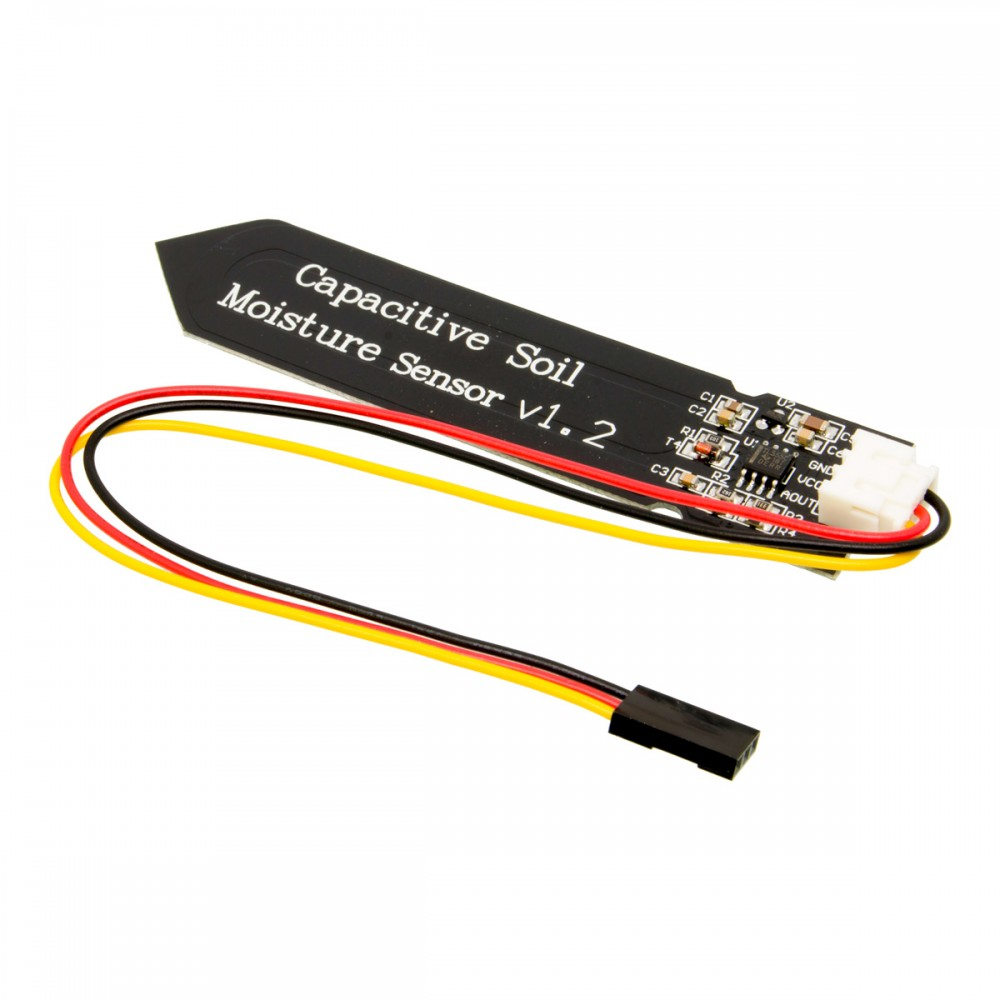
\includegraphics[height=10cm, width=\textwidth, keepaspectratio]{Imagenes/soilcapacitivesensor.jpg}
    \caption{Sensor de humedad de suelo capacitivo.}
    \Fuente{\cite{foto_sensor_suelo}}
\end{figure}

\subsubsection{Modulo de conversion Analogico a Digital}
Para la adquisición de señales analógicas y la optimización de los recursos de hardware, se seleccionó el circuito integrado PCF8591. Esta elección se justifica por su capacidad para expandir el sistema mediante cuatro entradas analógicas (ADC) de 8 bits que resultan suficientes para las tareas requeridas, utilizando únicamente dos líneas de comunicación gracias al protocolo I2C (\texttt{SDA} y \texttt{SCL}). Esta arquitectura periférica evita la saturación de los pines del microcontrolador principal, reservándolos para tareas críticas de actuación. Adicionalmente, el dispositivo ofrece la flexibilidad de configurar sus canales en modo diferencial para mitigar el ruido electromagnético en trayectos largos de cableado, y sus pines de direccionamiento por hardware (\texttt{A0}, \texttt{A1} y \texttt{A2}) garantizan la escalabilidad del sistema, permitiendo acoplar múltiples módulos en el mismo bus de datos sin requerir líneas de control adicionales. 
Gracias a estas caracteristicas y por su bajo coste y disponibilidad en el mercado se selecciono ese conversor.

\subsection{Alimentacion complementaria}
Con el propósito de energizar de manera dedicada los actuadores mecánicos, hídricos y las etapas de conmutación de potencia del sistema, se integró una fuente de alimentación conmutada de arquitectura avanzada extendida manufacturada por la marca Eurocase. La incorporación de este componente se fundamentó en un criterio metodológico de optimización de recursos preexistentes y minimización de costos operativos, aprovechando la disponibilidad inmediata del equipo en el laboratorio de desarrollo. Si bien los parámetros nominales de potencia de una fuente de este tipo exceden los requerimientos de consumo neto del prototipo, representando un sobredimensionamiento de la capacidad de corriente, su adopción evitó la adquisición de nuevos suministros comerciales sin comprometer la eficiencia. Asimismo, el dispositivo proporciona la ventaja tecnológica de entregar múltiples rieles de tensión estabilizados de forma simultánea, una característica que dota al sistema de versatilidad para futuras expansiones.

\subsection{Actuadores}
\subsubsection{Luces para el cultivo}
Para el sistema de iluminación artificial y estimulación del desarrollo vegetal, se implementó un panel LED para cultivo indoor de 50~W (marca Practiled). La elección de esta luminaria se justifica por su diseño espectral optimizado para la fotosíntesis, el cual concentra sus picos de emisión en las longitudes de onda de 450~nm (espectro azul) y 650~nm (espectro rojo), interactuando de manera directa con las clorofilas A y B para potenciar las fases de crecimiento vegetativo y floración. A su vez el módulo cuenta con protecciones contra sobretensión, sobrecorriente y un sensor de sobrecalentamiento crítico para el confinamiento del cultivo. Asimismo, cuenta con un grado de protección IP65 que garantiza su estanqueidad y resistencia frente a la alta humedad y salpicaduras derivadas del riego automatizado, operando con un regulador de voltaje interno que asegura una potencia constante y una alta eficiencia energética (clase A++). Debido a las caracteristicas mencionadas y su bajo coste en comparacion con otras opciones del mercado lo convirtieron en la opcion ideal para este proyecto.

\subsubsection{Bomba para riego}
Para el accionamiento del sistema de riego, se seleccionó una bomba periférica presurizadora de corriente continua (modelo Kushiro BPYK12). El parámetro determinante para esta elección fue su altura máxima de elevación de 2 metros, magnitud hidrodinámica que supera con holgura el nivel físico de la maceta, garantizando un suministro hídrico eficiente y sin caídas de presión hasta el estrato superior del cultivo. Desde la perspectiva de la integración electrónica y la seguridad, su operación a una tensión nominal de $12\text{ V}$ resulta fundamental para minimizar los riesgos de electrocución en un entorno caracterizado por alta humedad, facilitando además su control lógico mediante etapas de potencia estándar (relé) comandadas por el microcontrolador. Asimismo, su capacidad para entregar un caudal máximo de $3{,}8\text{ l/min}$ a una presión de trabajo de $2{,}5\text{ bar}$ es idónea para presurizar las líneas de riego sin generar caudales excesivos que inunden la zona radicular. Por último, su arquitectura mecánica, que incorpora un impulsor de bronce y un cuerpo de aluminio, proporciona una alta resistencia a la oxidación, asegurando la vida útil del actuador al operar con agua limpia.

\subsubsection{Valvulas solenoides}
Con el propósito de ejecutar la dosificación hídrica de manera precisa y dar cumplimiento al criterio de gestión sustentable del recurso hídrico, se implementaron emisores de riego localizado con una capacidad nominal máxima de 80 litros por hora. La integración física de estos componentes en la red de distribución se realiza de forma directa sobre la línea de conducción principal, efectuando un punzonado calibrado en la pared de la manguera de polietileno. Los goteros se introducen a presión dentro de esta perforación mediante un acoplamiento por interferencia mecánica, aprovechando las propiedades elásticas del material polimérico para asegurar la estanqueidad total del nodo y prevenir caídas de presión en el circuito. Estos dispositivos operan como actuadores pasivos finales y cuentan con un mecanismo de regulación helicoidal que permite modificar la sección transversal del conducto interno mediante obturación mecánica, optimizando la respuesta del lazo de irrigación automatizado.

\subsubsection{Goteros}
Con el propósito de ejecutar la dosificación hídrica de manera precisa y dar cumplimiento al criterio metodológico de gestión sustentable del recurso hídrico, se implementaron emisores de riego localizado con una capacidad nominal máxima de 80 litros por hora. Estos dispositivos operan como actuadores pasivos finales y cuentan con un mecanismo de regulación helicoidal que permite modificar la sección transversal del conducto interno mediante obturación mecánica. Esta capacidad de ajuste resulta crítica para la calibración del sistema, debido a que permite ecualizar la pérdida de carga en la red de distribución, garantizando que el coeficiente de descarga sea uniforme en todas las estaciones de cultivo y optimizando la respuesta del lazo de irrigación automatizado.
\begin{figure}[H]
    \centering
    \begin{minipage}{0.48\textwidth}
        \centering
        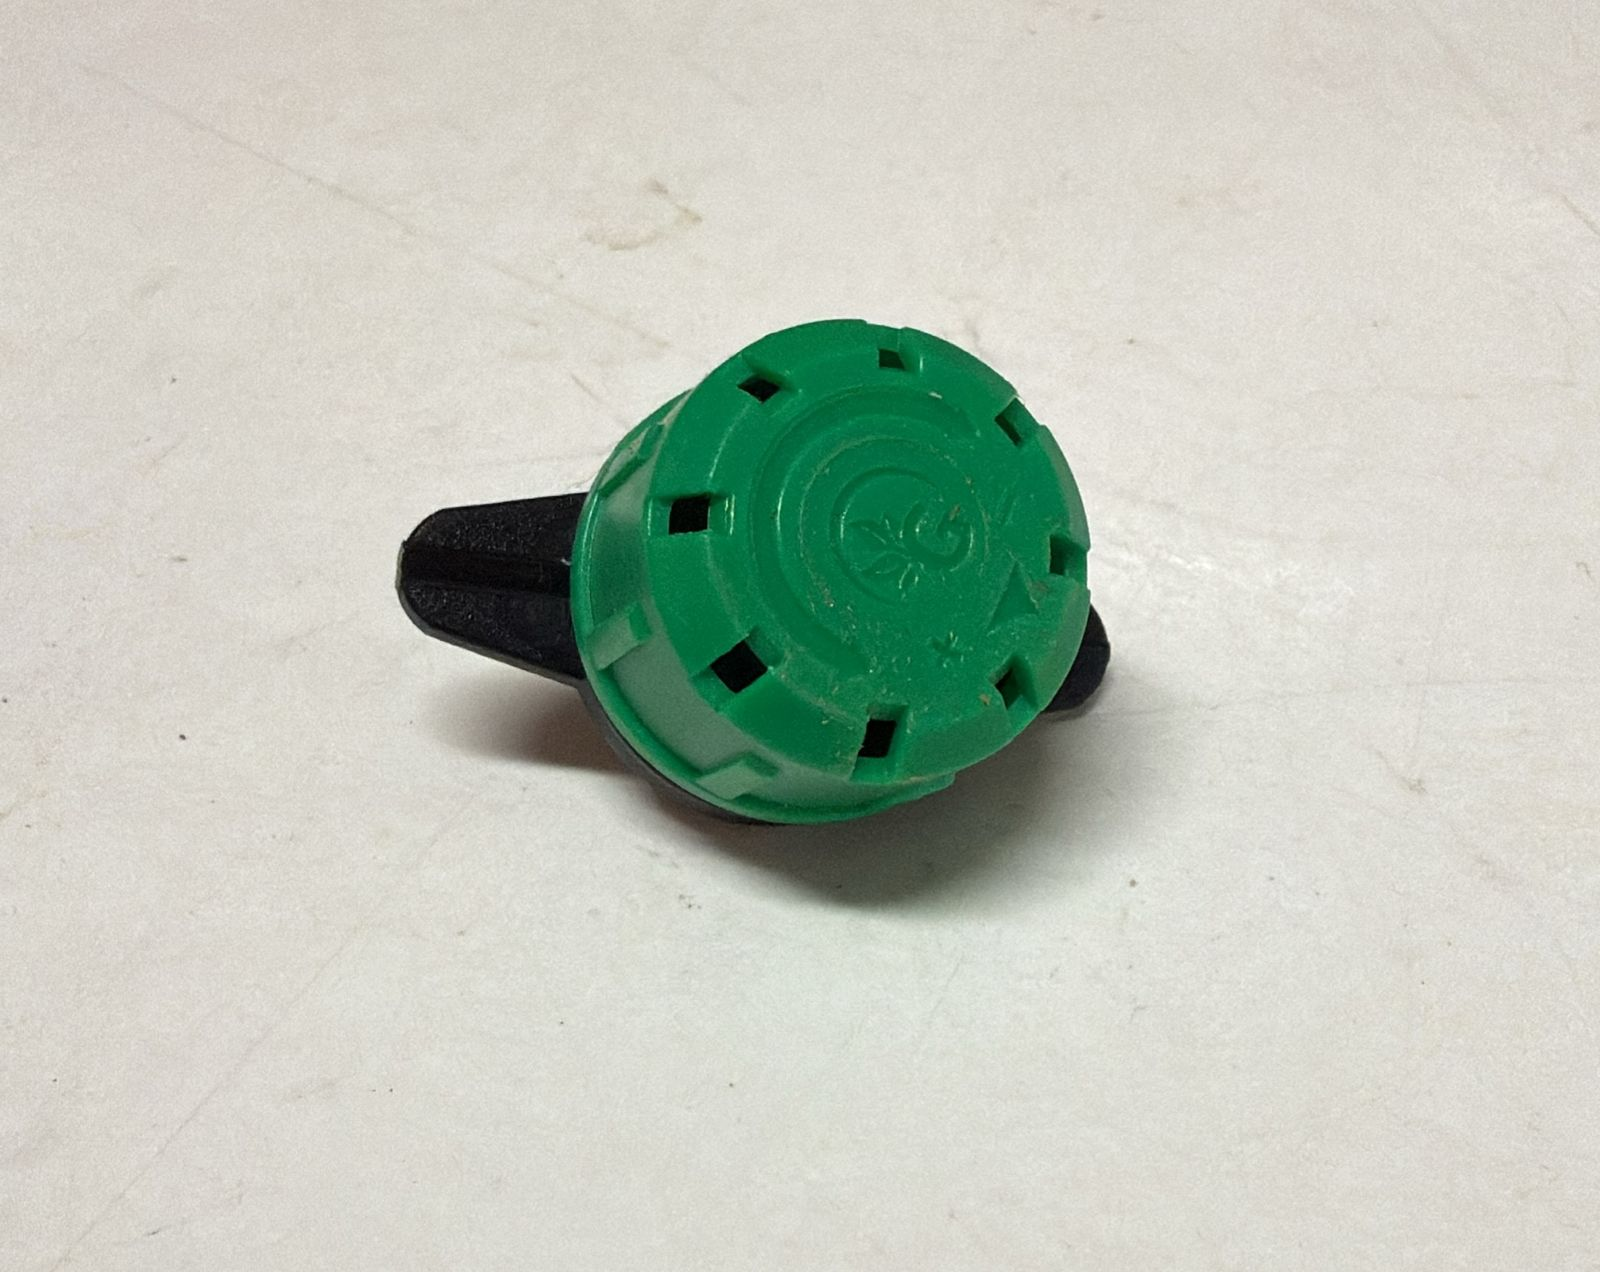
\includegraphics[height=10cm, width=\textwidth, keepaspectratio]{Imagenes/regador1.jpeg}
    \end{minipage}
    \hfill
    \begin{minipage}{0.48\textwidth}
        \centering
        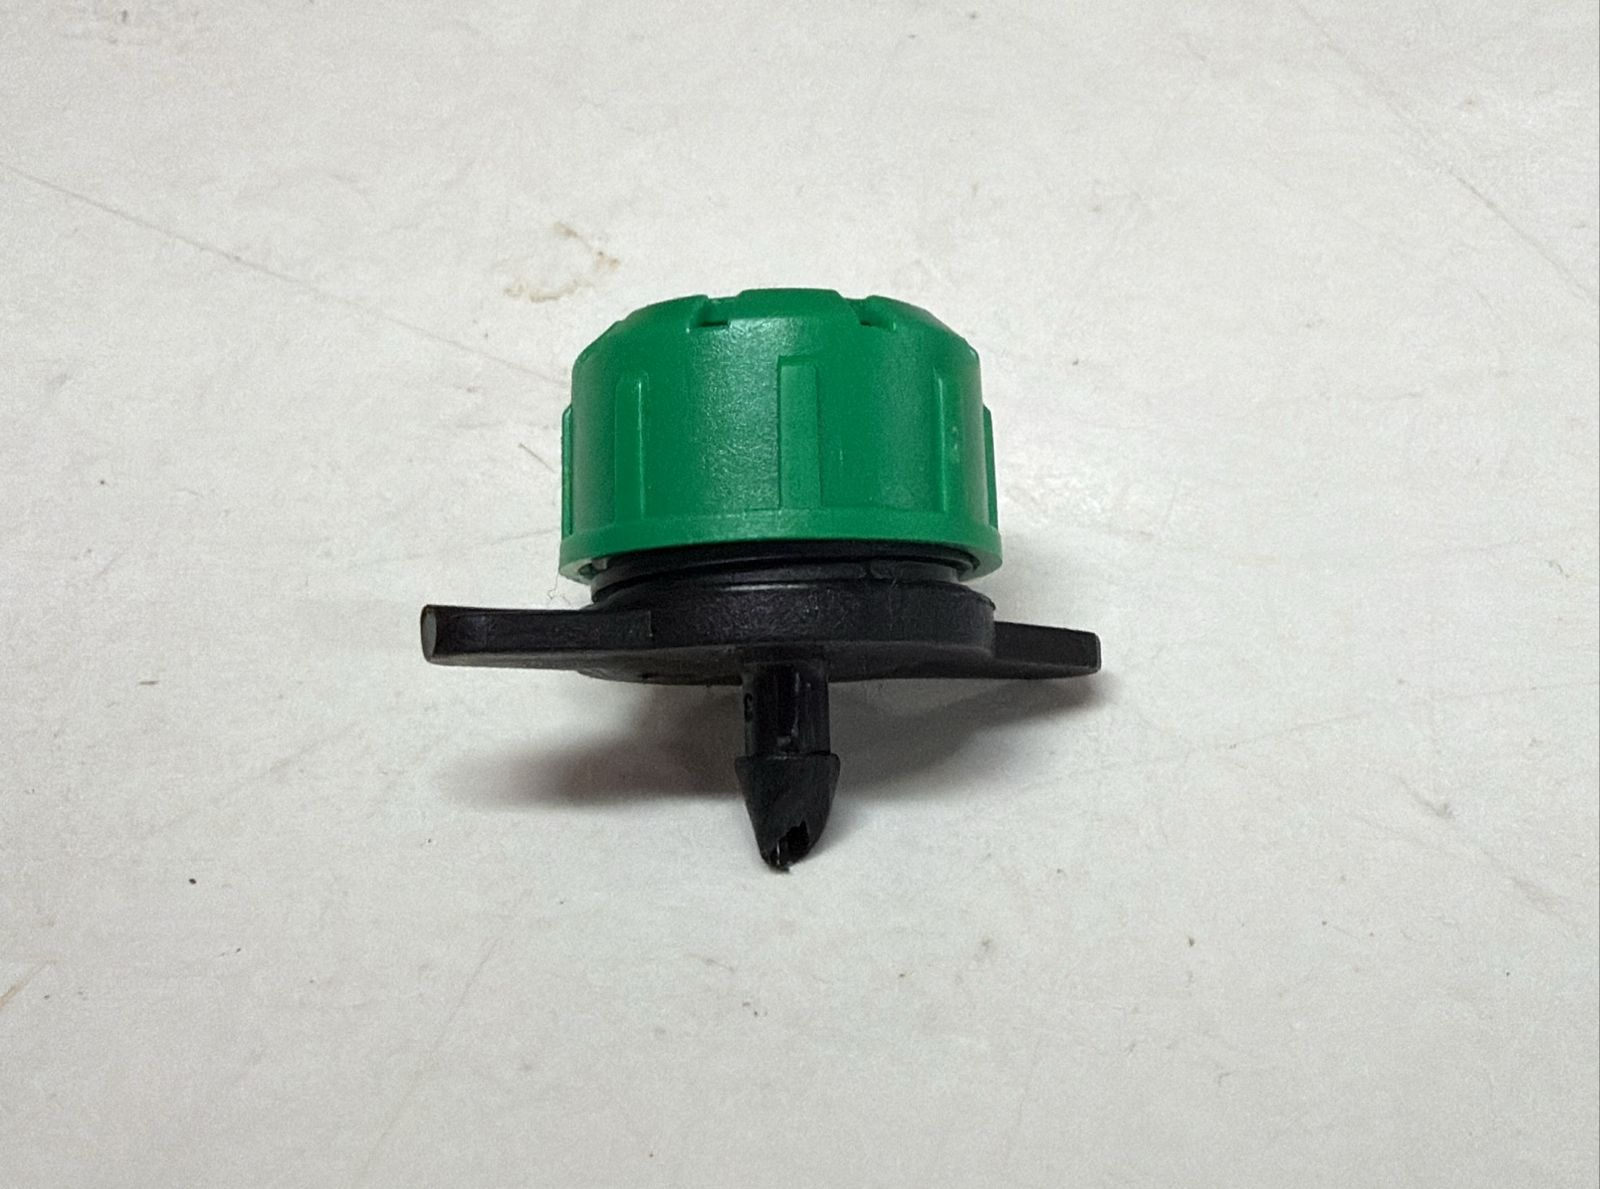
\includegraphics[height=10cm, width=\textwidth, keepaspectratio]{Imagenes/regador2.jpeg}
    \end{minipage}
    \caption{Goteros.}
    \Fuente{propia.}
\end{figure}

\subsection{Etapa de Potencia: Relés Electromecánicos y de Estado Sólido}
Para la gestión energética de los actuadores del sistema (luces, bomba hidráulica y válvulas solenoides), fue necesaria la implementación de módulos de relés, seleccionando tecnologías específicas según la naturaleza de la carga y el tipo de corriente a conmutar.
Por un lado, para el control de los paneles lumínicos, se optó por un módulo de relés de estado sólido (SSR) de dos canales con componentes OMRON. La elección de esta tecnología se justifica debido a que su etapa de salida está diseñada estrictamente para operar en corriente alterna (soportando hasta 240 VCA y 2 A). Al carecer de partes móviles, el SSR elimina la inercia mecánica, lo que permite realizar conmutaciones de encendido y apagado a gran velocidad sin sufrir fatiga ni desgaste físico a largo plazo. Adicionalmente, este módulo incorpora fusibles resistivos en su salida, añadiendo una capa de protección eléctrica fundamental para resguardar la integridad de las luminarias que son un elemento imprescindible del proyecto.
Por otro lado, para gobernar la bomba hidráulica y las válvulas solenoides (las cuales operan con corriente continua a 12 V) se implementó un módulo de relés electromecánicos de ocho canales. Esta decisión se fundamenta en la alta capacidad de manejo de corriente de sus contactos, los cuales soportan hasta 10 A a 30 VCC, resultando idóneos para absorber los picos de corriente transitorios que demandan las cargas inductivas (motores y electroimanes) durante su arranque. Un factor crítico para la elección de esta placa fue la integración de optoacopladores en sus entradas, esto garantiza un aislamiento galvánico completo entre la etapa de potencia y la lógica de control (5 V), protegiendo al microcontrolador frente a ruidos eléctricos o corrientes inversas generadas por las bobinas de los actuadores hidráulicos al desenergizarse.

\section{Diseños de piezas en 3D} 

Durante el desarrollo del proyecto, se diseñaron múltiples elementos mediante modelado 3D para facilitar la integración física de los sensores, los periféricos y demás componentes del sistema. Para esta tarea se empleó principalmente el software CAD Tinkercad, seleccionado por su entorno de diseño intuitivo y la versatilidad de sus herramientas.
Para la fabricación de las piezas se hizo uso del laminador Cura Slicer, y los parámetros utilizados fueron orientados a maximizar la estanqueidad y la resistencia mecánica. En particular, se utilizó un espesor de pared de 3 mm, correspondiente a 5 líneas de pared, lo que permite generar una estructura externa robusta y continúa, reduciendo la posibilidad de filtraciones a través de las capas.
Se adoptó una densidad de relleno del 100 porciento, con el objetivo de eliminar cavidades internas que puedan favorecer el paso de agua, garantizando así una mayor impermeabilidad de la pieza. Asimismo, se configuraron 8 capas superiores e inferiores, reforzando las superficies horizontales y contribuyendo a un cierre más efectivo del volumen impreso.
La altura de capa se fijó en 0,20 mm, valor que representa un compromiso adecuado entre tiempo de impresión y calidad superficial, permitiendo una correcta adhesión entre capas. Por su parte, el flujo de material se ajustó al 103 porciento, lo que incrementa ligeramente la cantidad de material extruido, favoreciendo el relleno de posibles microespacios entre trayectorias y mejorando el sellado general.
En cuanto a las condiciones térmicas, se empleó una temperatura de extrusión de 207 °C, adecuada para el material PLA utilizado, asegurando una correcta fusión entre capas. Finalmente, la velocidad de impresión se estableció en 40 mm/s, valor moderado que contribuye a una deposición más controlada del material, mejorando la adherencia y reduciendo la probabilidad de defectos que puedan comprometer la estanqueidad.

\subsubsection{Soporte para sensores} 
El diseño de esta pieza tuvo como objetivo principal proporcionar un alojamiento seguro y estable para realizar las primeras pruebas de los módulos de sensado. Esta fijación garantiza que las mediciones de las variables ambientales se realicen de manera correcta y repetible, evitando cualquier disposición aleatoria dentro del sistema. La estructura cuenta con aberturas dimensionadas para el encastre preciso de cada sensor e incorpora canalizaciones internas específicas para el guiado y protección del cableado.

\begin{figure}[H]
    \centering
    % --- Imagen 1 ---
    \begin{minipage}{0.31\textwidth}
        \centering
        \includegraphics[height=10cm, width=\textwidth, keepaspectratio]{Imagenes/imagen16.png}
    \end{minipage}
    \hfill
    % --- Imagen 2 ---
    \begin{minipage}{0.31\textwidth}
        \centering
        \includegraphics[height=10cm, width=\textwidth, keepaspectratio]{Imagenes/imagen17.png}
    \end{minipage}
    \hfill
    % --- Imagen 3 ---
    \begin{minipage}{0.31\textwidth}
        \centering
        \includegraphics[height=10cm, width=\textwidth, keepaspectratio]{Imagenes/imagen18.png}
    \end{minipage}

    \caption{Primer diseno de soporte para sensores}
    \Fuente{propia.}
    \label{fig:detalles_3d_triple2}
\end{figure}

Luego, la implementacion fisica:

\begin{figure}[H]
    \centering
    % --- Imagen 1 ---
    \begin{minipage}{0.31\textwidth}
        \centering
        \includegraphics[height=10cm, width=\textwidth, keepaspectratio]{Imagenes/imagen3.png}
    \end{minipage}
    \hfill
    % --- Imagen 2 ---
    \begin{minipage}{0.31\textwidth}
        \centering
        \includegraphics[height=10cm, width=\textwidth, keepaspectratio]{Imagenes/imagen9.png}
    \end{minipage}
    \hfill
    % --- Imagen 3 ---
    \begin{minipage}{0.31\textwidth}
        \centering
        \includegraphics[height=10cm, width=\textwidth, keepaspectratio]{Imagenes/imagen10.png}
    \end{minipage}

    \caption{Implementacion fisica.}
    \Fuente{propia.}
    \label{fig:detalles_3d_triple1}
\end{figure}

\subsubsection{Soporte para manguera}
Se diseñó una pieza vertical para su inserción en el suelo, con un sistema superior de sujeción que fija la manguera, permitiendo un trazado del circuito ordenado y definido.

\begin{figure}[H]
    \centering
    \begin{minipage}{0.48\textwidth}
        \centering
        \includegraphics[height=10cm, width=\textwidth, keepaspectratio]{Imagenes/imagen1.png}
    \end{minipage}
    \hfill
    \begin{minipage}{0.48\textwidth}
        \centering
        \includegraphics[height=10cm, width=\textwidth, keepaspectratio]{Imagenes/imagen8.png}
    \end{minipage}
    \caption{Soporte para mangueras.}
    \Fuente{propia.}
\end{figure}

\subsubsection{Acople Y} 
Para la unión de las mangueras, se diseñó un acople que permite vincularlas optimizando el espacio disponible y mejorando su organización.
\begin{figure}[H]
    \centering
    \begin{minipage}{0.48\textwidth}
        \centering
        \includegraphics[height=10cm, width=\textwidth, keepaspectratio]{Imagenes/imagen15.png}
    \end{minipage}
    \hfill
    \begin{minipage}{0.48\textwidth}
        \centering
        \includegraphics[height=10cm, width=\textwidth, keepaspectratio]{Imagenes/imagen1.jpeg}
    \end{minipage}
    \caption{Conector Y.}
    \Fuente{propia.}
\end{figure}

\subsubsection{Filtro de desagüe v1} 
Inicialmente, se diseñó un filtro con acople para manguera de ½ pulgada, con el objetivo de retener la tierra y conducir el agua a través del orificio realizado en la madera hasta el contenedor.
\begin{figure}[H]
    \centering
    \begin{minipage}{0.48\textwidth}
        \centering
        \includegraphics[height=10cm, width=\textwidth, keepaspectratio]{Imagenes/imagen2.png}
    \end{minipage}
    \hfill
    \begin{minipage}{0.48\textwidth}
        \centering
        \includegraphics[height=10cm, width=\textwidth, keepaspectratio]{Imagenes/imagen7.png}
    \end{minipage}
    \caption{Desagüe v1.}
    \Fuente{propia.}
\end{figure}

\subsubsection{Filtro de desagüe v2}
Debido a que la primera implementación no funcionó según lo esperado, se realizaron modificaciones. Se desarrolló un sistema roscado que permite ejercer presión sobre la madera, logrando un mejor sellado y evitando filtraciones sin perder capacidad de filtrado. Además, se mantuvo la conexión para manguera de ½ pulgada y se incorporó una forma curvada en la pieza que permite disponer la manguera de manera más compacta, favoreciendo el flujo de agua sin restricciones.

\begin{figure}[H]
    \centering
    % --- Imagen 1 ---
    \begin{minipage}{0.31\textwidth}
        \centering
        \includegraphics[height=10cm, width=\textwidth, keepaspectratio]{Imagenes/imagen11.png}
    \end{minipage}
    \hfill
    % --- Imagen 2 ---
    \begin{minipage}{0.31\textwidth}
        \centering
        \includegraphics[height=10cm, width=\textwidth, keepaspectratio]{Imagenes/imagen13.png}
    \end{minipage}
    \hfill
    % --- Imagen 3 ---
    \begin{minipage}{0.31\textwidth}
        \centering
        \includegraphics[height=10cm, width=\textwidth, keepaspectratio]{Imagenes/imagen17.jpeg}
    \end{minipage}
    \caption{Desagüe v2.}
    \Fuente{propia.}
\end{figure}

\subsubsection{Soporte para ventilador} 
Se diseñaron soportes específicos para la sujeción de los ventiladores, orientados a maximizar la versatilidad del sistema de control ambiental. Estos componentes fueron proyectados para permitir una instalación dinámica, pudiendo desplazarse y fijarse en cualquier punto a lo largo del perímetro de la estructura de cultivo, según los requerimientos específicos de las especies vegetales o las fases del desarrollo fenológico.
Esta configuración ajustable no solo optimiza la circulación del flujo de aire y la disipación térmica, sino que también mejora la portabilidad del prototipo. Al permitir el desmontaje o reubicación rápida de los ventiladores, se facilita el traslado de los módulos y se minimiza el riesgo de daños mecánicos en los actuadores durante las maniobras de transporte o mantenimiento.

\begin{figure}[H]
    \centering
    \begin{minipage}{0.48\textwidth}
        \centering
        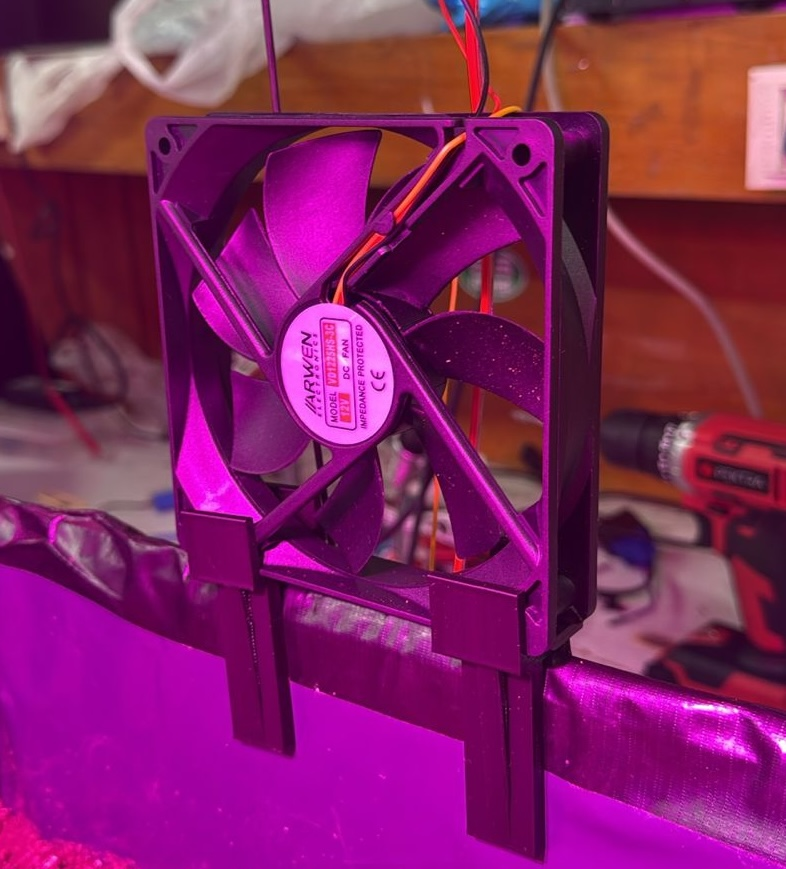
\includegraphics[width=\textwidth]{Imagenes/soporteventilador2.jpeg}
    \end{minipage}
    \hfill
    \begin{minipage}{0.48\textwidth}
        \centering
        \includegraphics[width=\textwidth]{Imagenes/soporteventilador1.png}
    \end{minipage}
    \caption{Soporte para ventilador.}
    \Fuente{propia.}
    \label{fig:soporte_mangueras}
\end{figure}

\subsubsection{Soporte para sensor de humedad y temperatura} 
Se diseñó un soporte específico para la integración del sensor DHT22. El diseño contempla un encapsulado con estructura reticular (tipo malla) que actúa como barrera física para resguardar el dispositivo frente a posibles salpicaduras de riego, acumulación de polvo e impactos mecánicos accidentales.
Esta configuración de "carcasa ventilada" es fundamental para asegurar la integridad del componente sin comprometer su funcionamiento; la porosidad del diseño permite la libre circulación del aire, garantizando que el sensor mantenga un tiempo de respuesta óptimo y continúe proporcionando lecturas de las variables ambientales con la precisión requerida por el sistema de control.

\begin{figure}[H]
    \centering
    \begin{minipage}{0.48\textwidth}
        \centering
        \includegraphics[width=\textwidth]{Imagenes/soportedht1.jpeg}
    \end{minipage}
    \hfill
    \caption{Soporte DHT22.}
    \Fuente{propia.}
    \label{fig:soporte_mangueras}
\end{figure}

\subsubsection{Soporte para sensor de iluminancia}
Para la correcta fijación del sensor de luz, se diseñaron soportes modulares basados en el principio de acoplamiento de los ventiladores del sistema. Estas estructuras permiten una reconfiguración posicional flexible dentro del entorno de cultivo, otorgando la versatilidad de retirar y reubicar los sensores en diferentes puntos estratégicos según los requerimientos lumínicos de la etapa fenológica de las plantas y la geometría del ambiente.
\begin{figure}[H]
    \centering
    \begin{minipage}{0.48\textwidth}
        \centering
        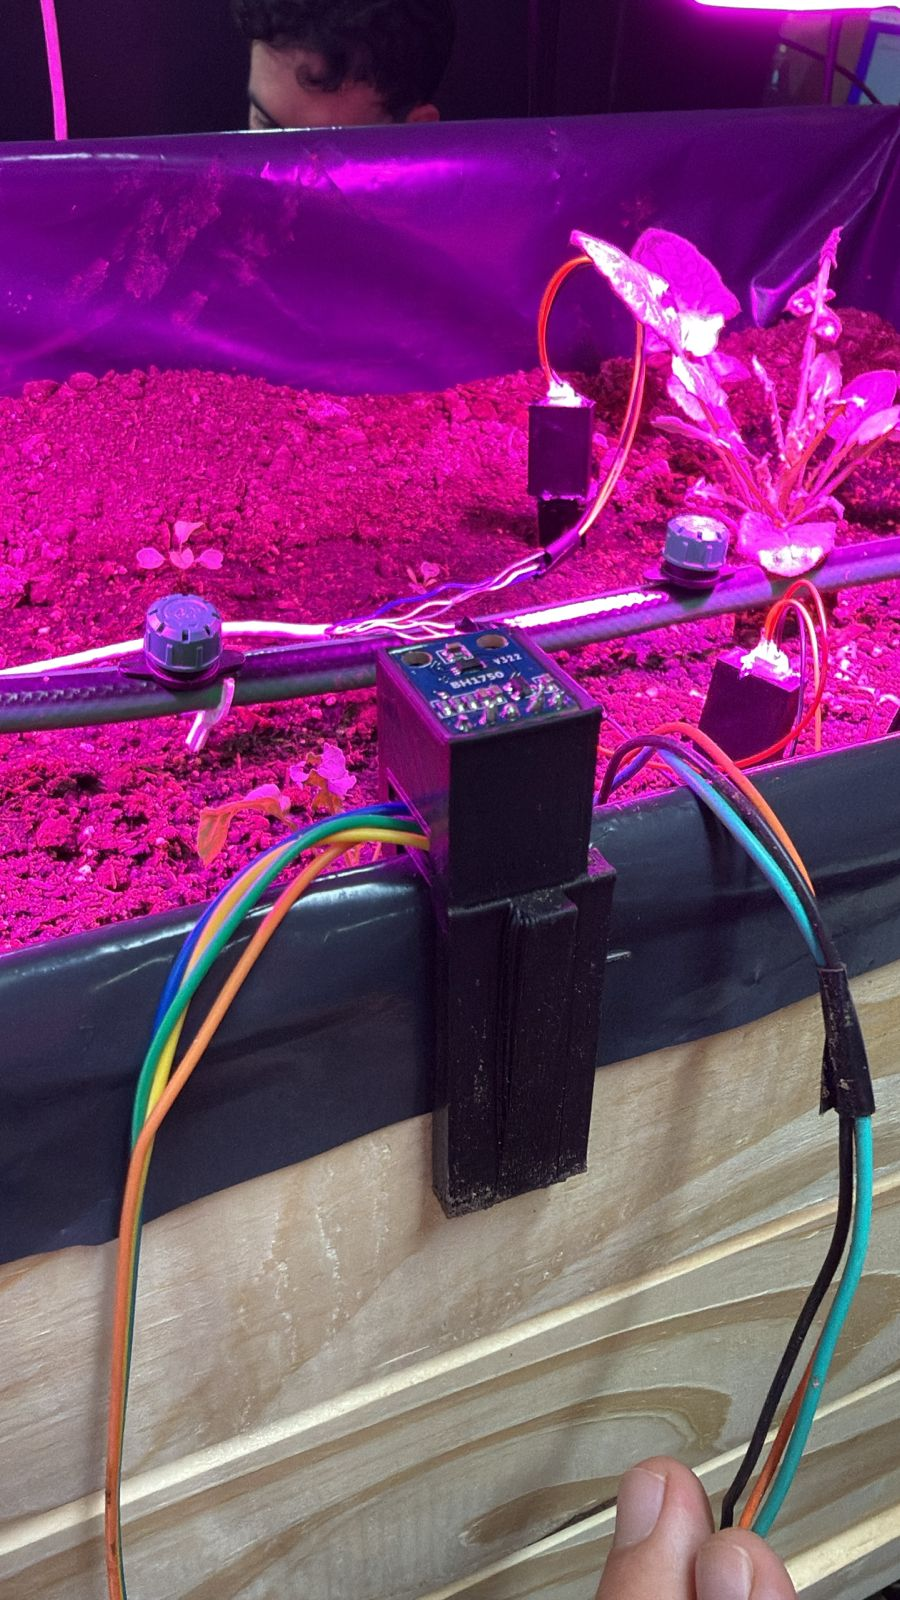
\includegraphics[width=\textwidth]{Imagenes/soportebh17501.png}
    \end{minipage}
    \hfill
    \begin{minipage}{0.48\textwidth}
        \centering
        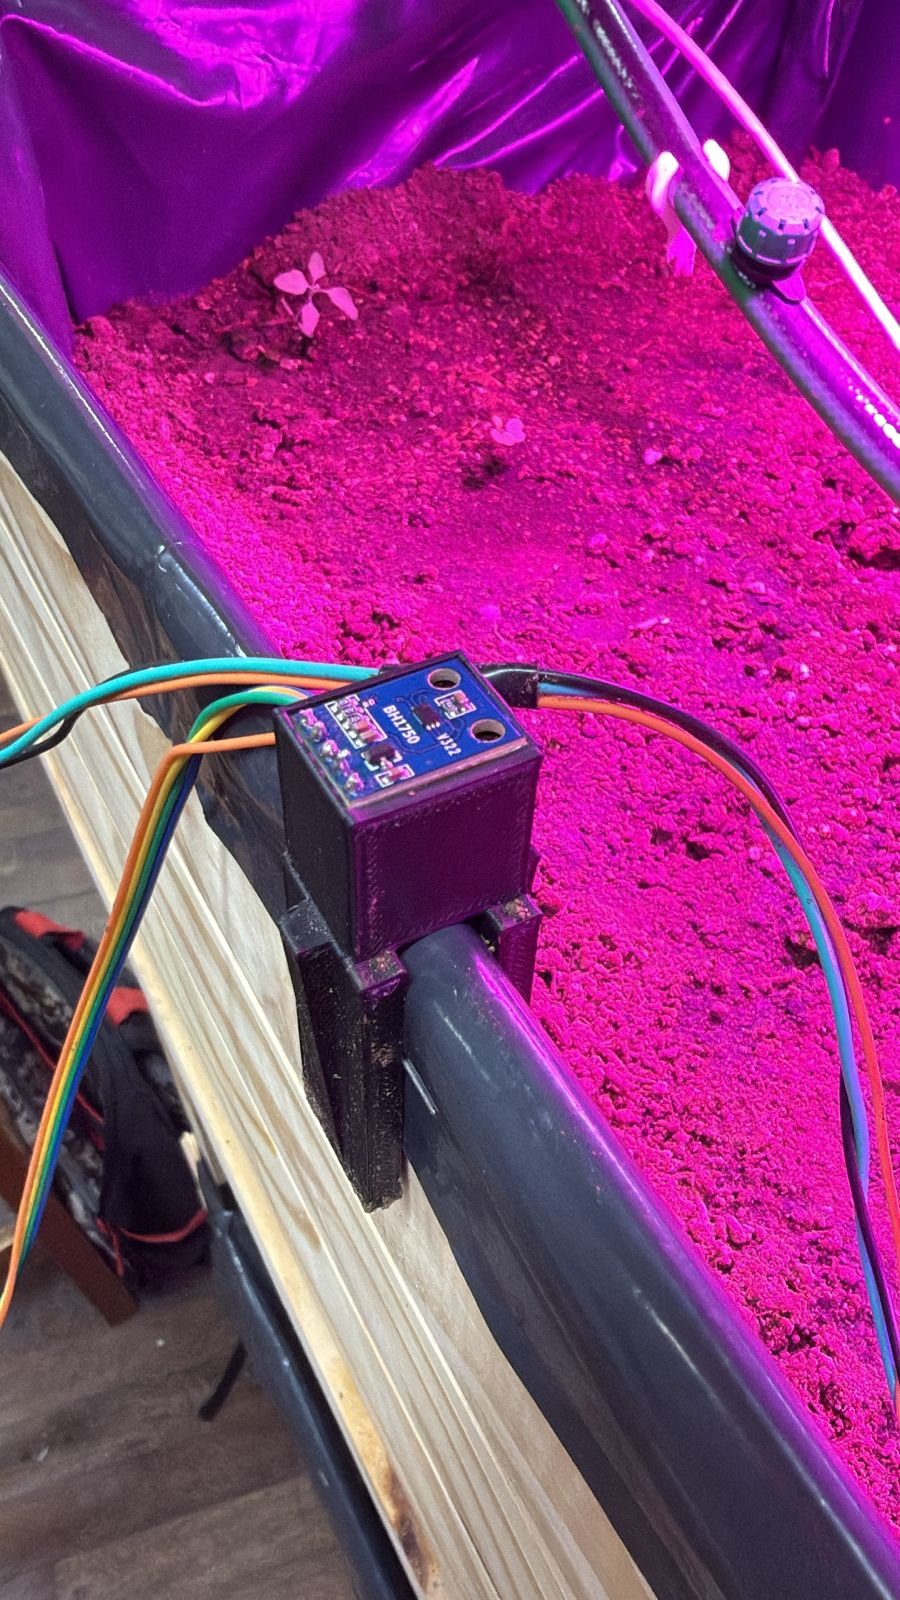
\includegraphics[width=\textwidth]{Imagenes/soportebh17502.jpeg}
    \end{minipage}
    \caption{Soporte para BH1750.}
    \Fuente{propia.}
    \label{fig:soporte_mangueras}
\end{figure}

\subsubsection{Covertor de proteccion para higrómetros} 
Para la impermeabilización de los sensores de humedad de suelo, se diseñaron carcasas de protección a medida con el propósito de aislar herméticamente sus componentes electrónicos sensibles. Asimismo, los puntos de acoplamiento mecánico y las vías de salida del cableado fueron sellados mediante la aplicación de silicona de alta resistencia, garantizando la estanqueidad del conjunto y previniendo filtraciones que pudieran degradar los circuitos durante la operación en sustratos húmedos.\begin{figure}[H]
    \centering
    \begin{minipage}{0.48\textwidth}
        \centering
        \includegraphics[width=\textwidth]{Imagenes/soportehigrometro1.jpeg}
    \end{minipage}
    \hfill
    \begin{minipage}{0.48\textwidth}
        \centering
        \includegraphics[width=\textwidth]{Imagenes/soportehigrometro2.jpeg}
    \end{minipage}
    \caption{Covertor para higrometro.}
    \Fuente{propia.}
    \label{fig:soporte_mangueras}
\end{figure}
Posteriormente a la vinculación y calibración del sensor, se inició la etapa de adecuación física orientada a la protección del circuito electrónico interno contra agentes ambientales. Con este propósito, se aplicó un polímero de silicona de alta rigidez dieléctrica sobre todas las uniones de la carcasa e interfaces de los conductores, estableciendo una barrera hermética contra la humedad. Esta acción de sellado resulta crítica en el diseño, dado que previene la infiltración de agua hacia las pistas de cobre y componentes activos, resguardando el sistema ante posibles derivaciones de corriente que degraden la linealidad de las lecturas analógicas o causen fallas catastróficas por cortocircuito en las etapas de alimentación.

\begin{figure}[H]
    \centering
    \begin{minipage}{0.48\textwidth}
        \centering
        \includegraphics[width=\textwidth]{Imagenes/Imperm_Sensor1.jpeg}
    \end{minipage}
    \hfill
    \begin{minipage}{0.48\textwidth}
        \centering
        \includegraphics[width=\textwidth]{Imagenes/Imperm_Sensor2.jpeg}
    \end{minipage}
    \caption{Proceso de impermeabilización del sensor.}
    \Fuente{propia.}
    \label{fig:soporte_mangueras}
\end{figure}

\section{Disposicion de las luminarias}
Para la instalación física del panel de espectro completo, se acondicionó la viga transversal de madera posicionada en el estrato superior de la estación de cultivo, integrando armellas de sujeción cerrada conocidas comercialmente como tornillos ojo. A través de estos componentes mecánicos se enhebran las eslingas de acero que suspenden el artefacto lumínico, estableciendo una matriz de fijación redundante. La distribución geométrica de estos anclajes se calculó con el propósito operativo de regular de forma manual el distanciamiento vertical entre el foco y el ápice del dosel vegetal; esta modularidad posicional permite manipular de manera directa la densidad de flujo fotónico y la carga térmica por radiación que incide sobre las especies bajo ensayo. En la etapa de germinación, posterior a la siembra, las luminarias se configuran en su cota altimétrica mínima, optimizando la transferencia de energía electromagnética necesaria para estimular los fotorreceptores iniciales de las plántulas. A continuación, se ilustra la resolución constructiva descrita para el soporte lumínico:
\begin{figure}[H]
    \centering
    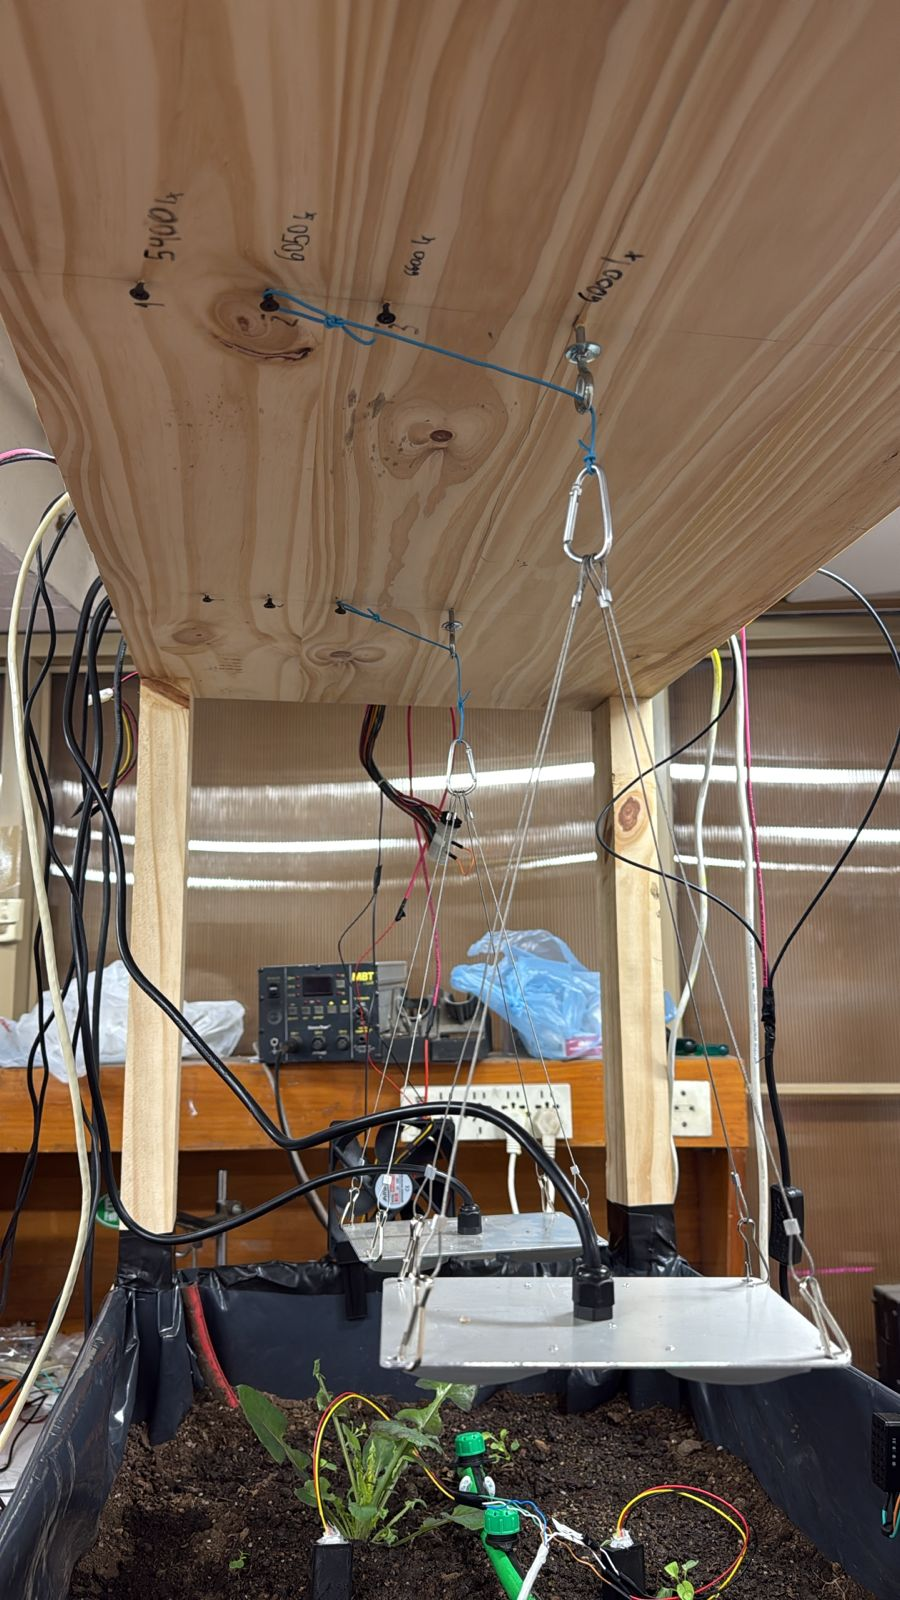
\includegraphics[height=10cm, width=\textwidth, keepaspectratio]{Imagenes/luminaria.jpeg}
    \caption{Disposicion de las luminarias.}
    \Fuente{propia.}
\end{figure}

\section{Disposicion de hardware}
Con el propósito de alojar los módulos de control y procesamiento del sistema (tales como la unidad central Raspberry Pi 4, la placa de relés y los conversores analógico-digitales (ADC)), se definió una localización estratégica basada en criterios de accesibilidad, seguridad y optimización de las líneas de señal. Se optó por ubicar este núcleo de control en la zona superior de la estructura, logrando una posición equidistantemente centralizada que facilita el ruteado de los cables hacia los distintos sensores y actuadores del prototipo, minimizando a su vez el impacto visual y la interferencia estructural.
Esta disposición en altura aísla la electrónica crítica frente a riesgos mecánicos por manipulación directa o eventuales filtraciones y salpicaduras provenientes del subsistema hidráulico. Para garantizar un aislamiento eléctrico adecuado y protección contra humedad y polvo, la totalidad de los componentes se confinó dentro de un gabinete con sellado hermético. La interconexión con los periféricos externos se ejecutó mediante pasacables con prensacables (pasamuros), permitiendo el paso ordenado y seguro de los conductores sin comprometer el nivel de protección de la envolvente.
\begin{figure}[H]
    \centering
    \begin{minipage}{0.48\textwidth}
        \centering
        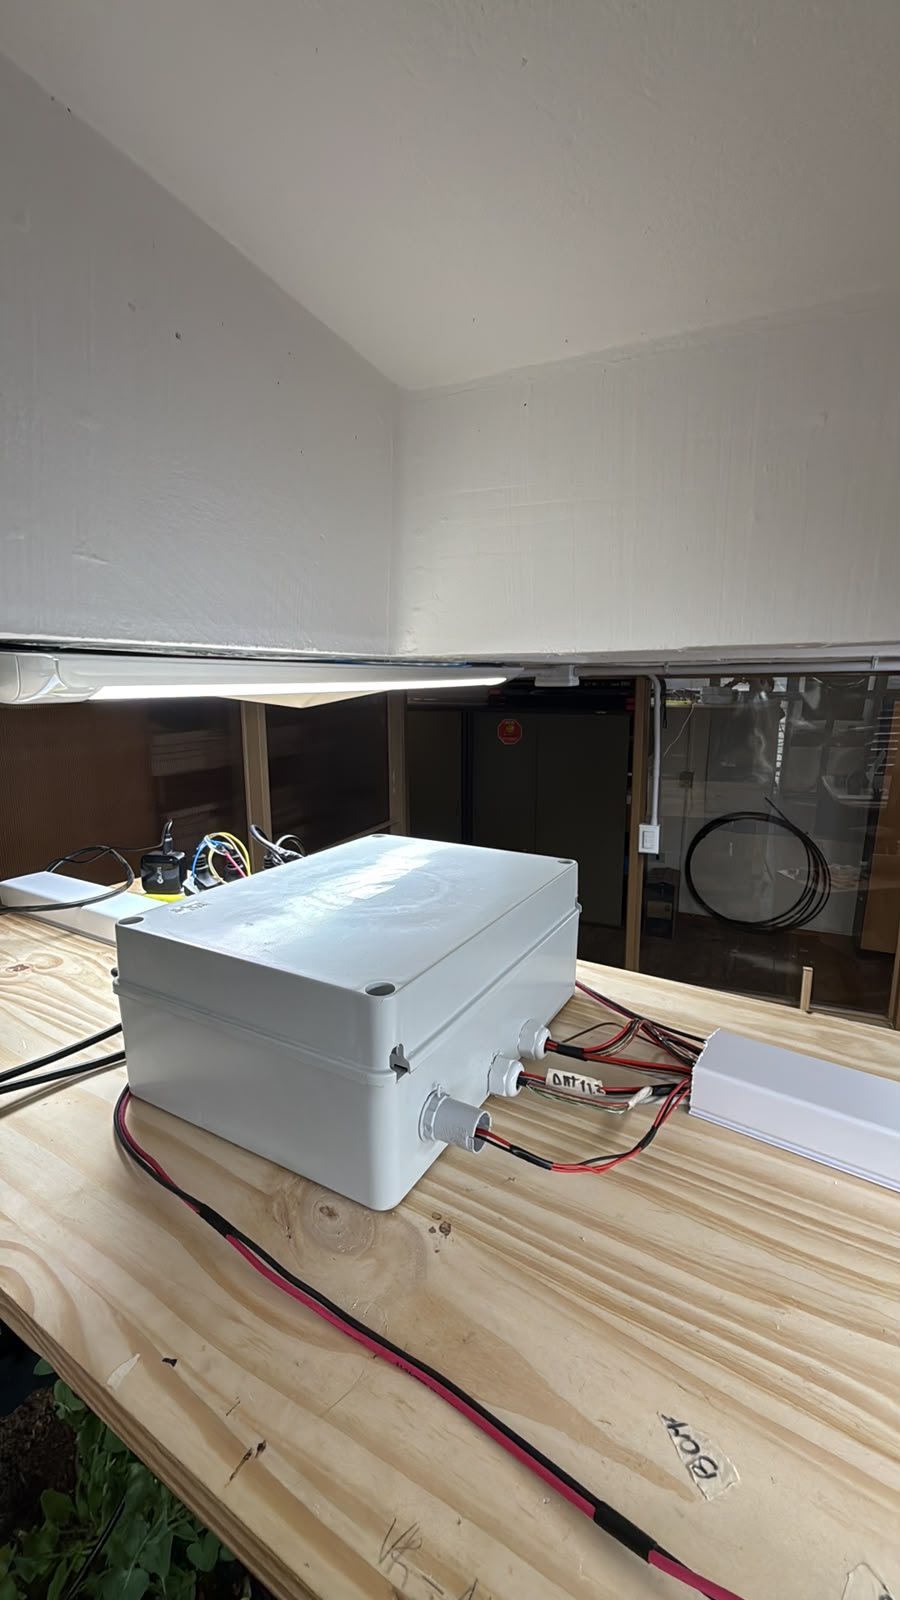
\includegraphics[width=\textwidth]{Imagenes/modulocentral1.jpeg}
    \end{minipage}
    \hfill
    \begin{minipage}{0.48\textwidth}
        \centering
        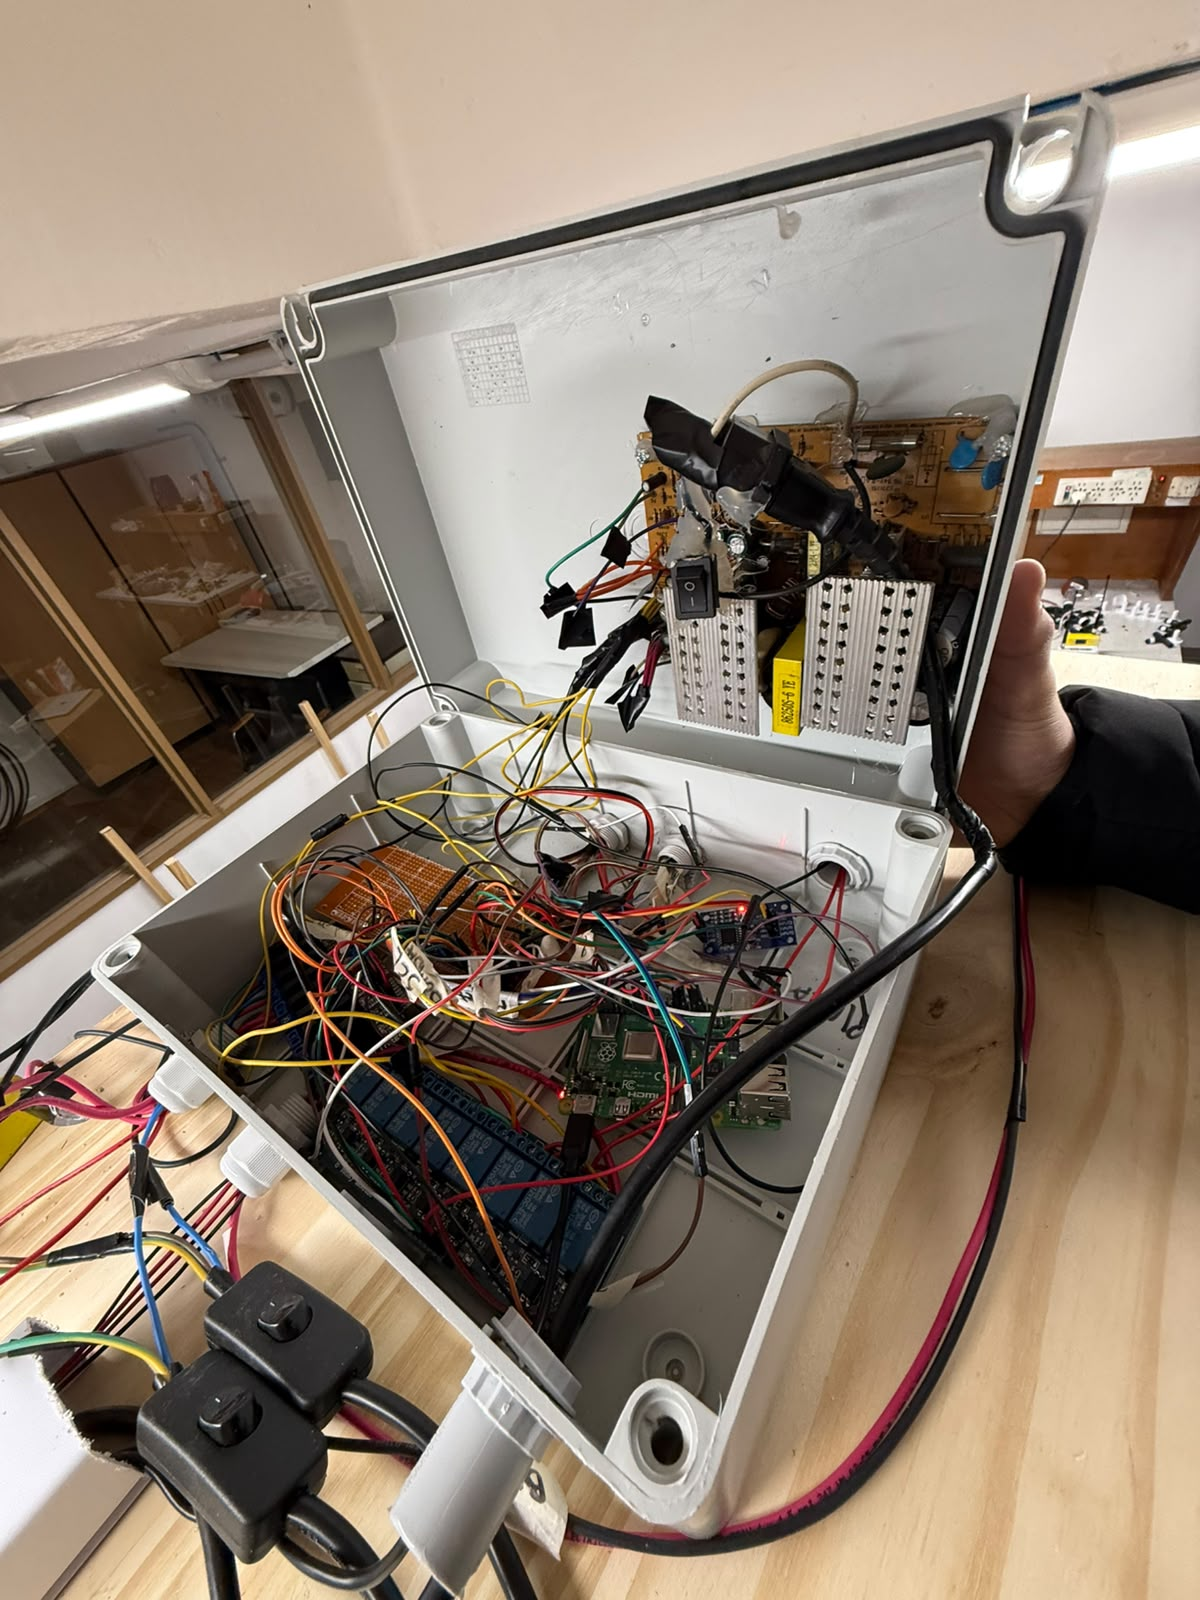
\includegraphics[width=\textwidth]{Imagenes/modulocentral2.jpeg}
    \end{minipage}
    \caption{Caja electrica estanca con componentes vitales del sistema.}
    \Fuente{propia.}
    \label{fig:soporte_mangueras}
\end{figure}

\section{Circuito de riego}
El subsistema de irrigación opera mediante un esquema de distribución selectiva alimentado por la electrobomba descrita en apartados anteriores. A través de un arreglo de válvulas solenoides, el firmware puede dirigir el flujo hídrico hacia un módulo o maceta en particular, según las requerimientos de humedad detectados por los sensores. La canalización principal se ejecutó utilizando tubos flexibles de 1/2 pulgada, dimensión seleccionada para garantizar un caudal óptimo de operación sin generar sobrepresiones en los acoples. En el tramo interno de cada contenedor se instalaron goteros autocompensados que liberan un caudal volumétrico constante por unidad de tiempo, logrando una distribución homogénea del recurso hídrico en la zona radicular.
\begin{figure}[H]
    \centering
    \begin{minipage}{0.48\textwidth}
        \centering
        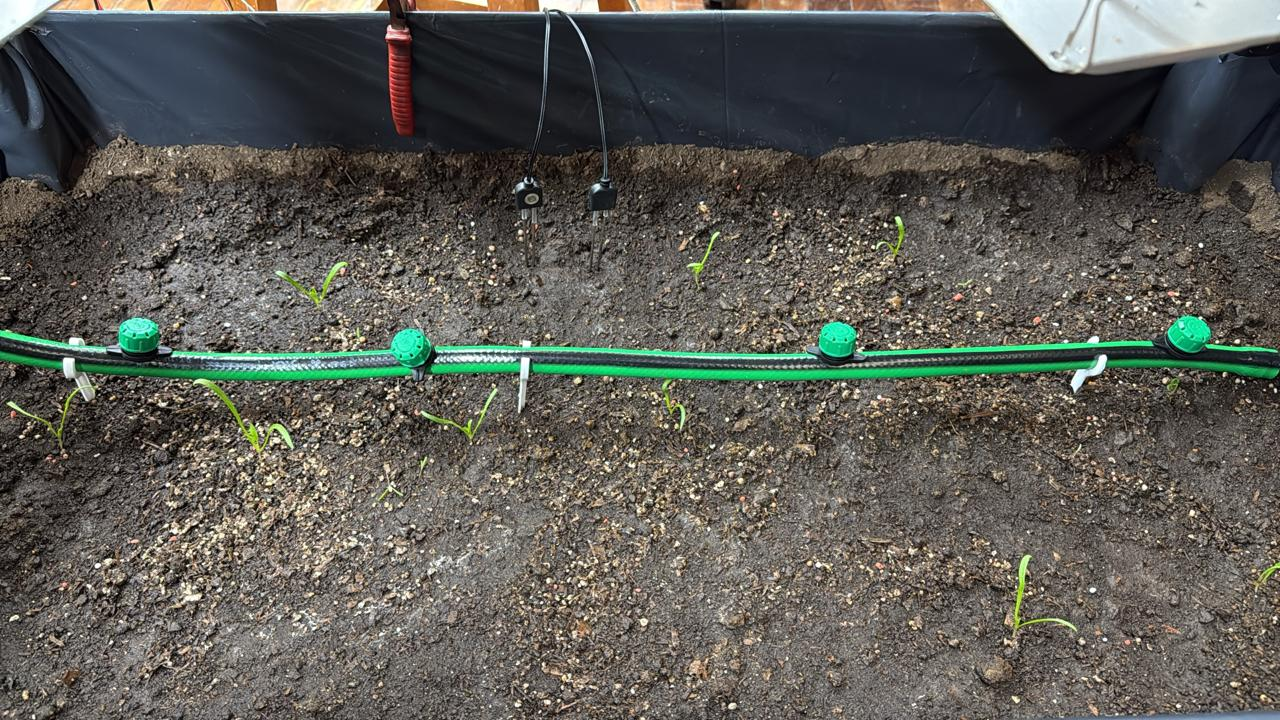
\includegraphics[width=\textwidth]{Imagenes/sistemariego.jpeg}
    \end{minipage}
    \hfill
    \begin{minipage}{0.48\textwidth}
        \centering
        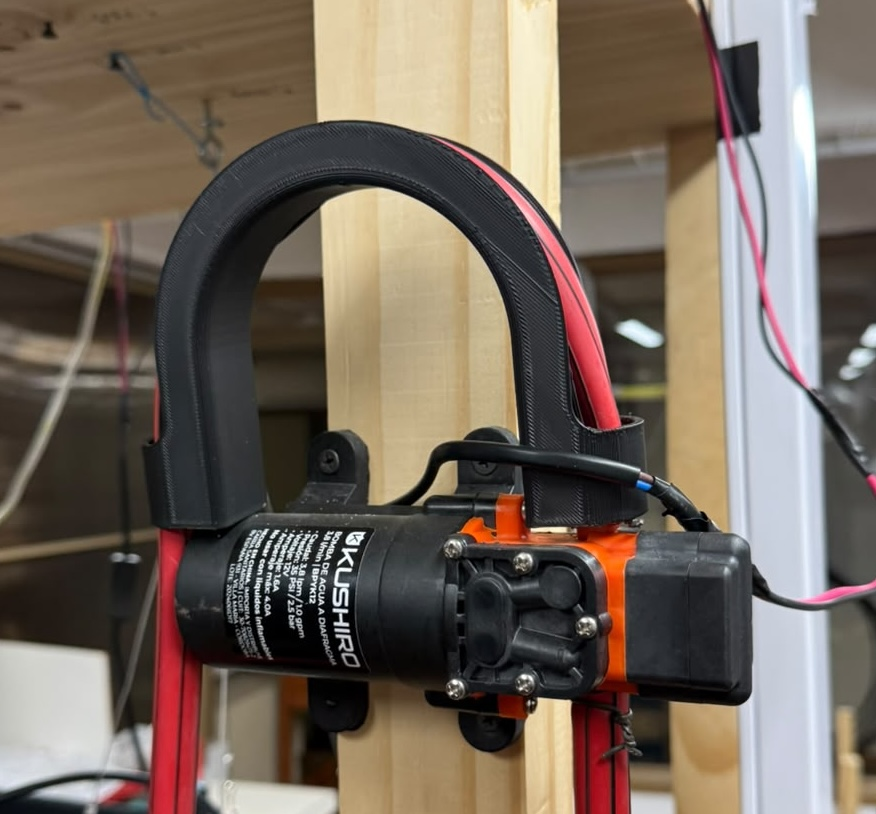
\includegraphics[width=\textwidth]{Imagenes/bomba.jpeg}
    \end{minipage}
    \caption{Sistema de riego.}
    \Fuente{propia.}
    \label{fig:soporte_mangueras}
\end{figure}
\begin{figure}[H]
    \centering
    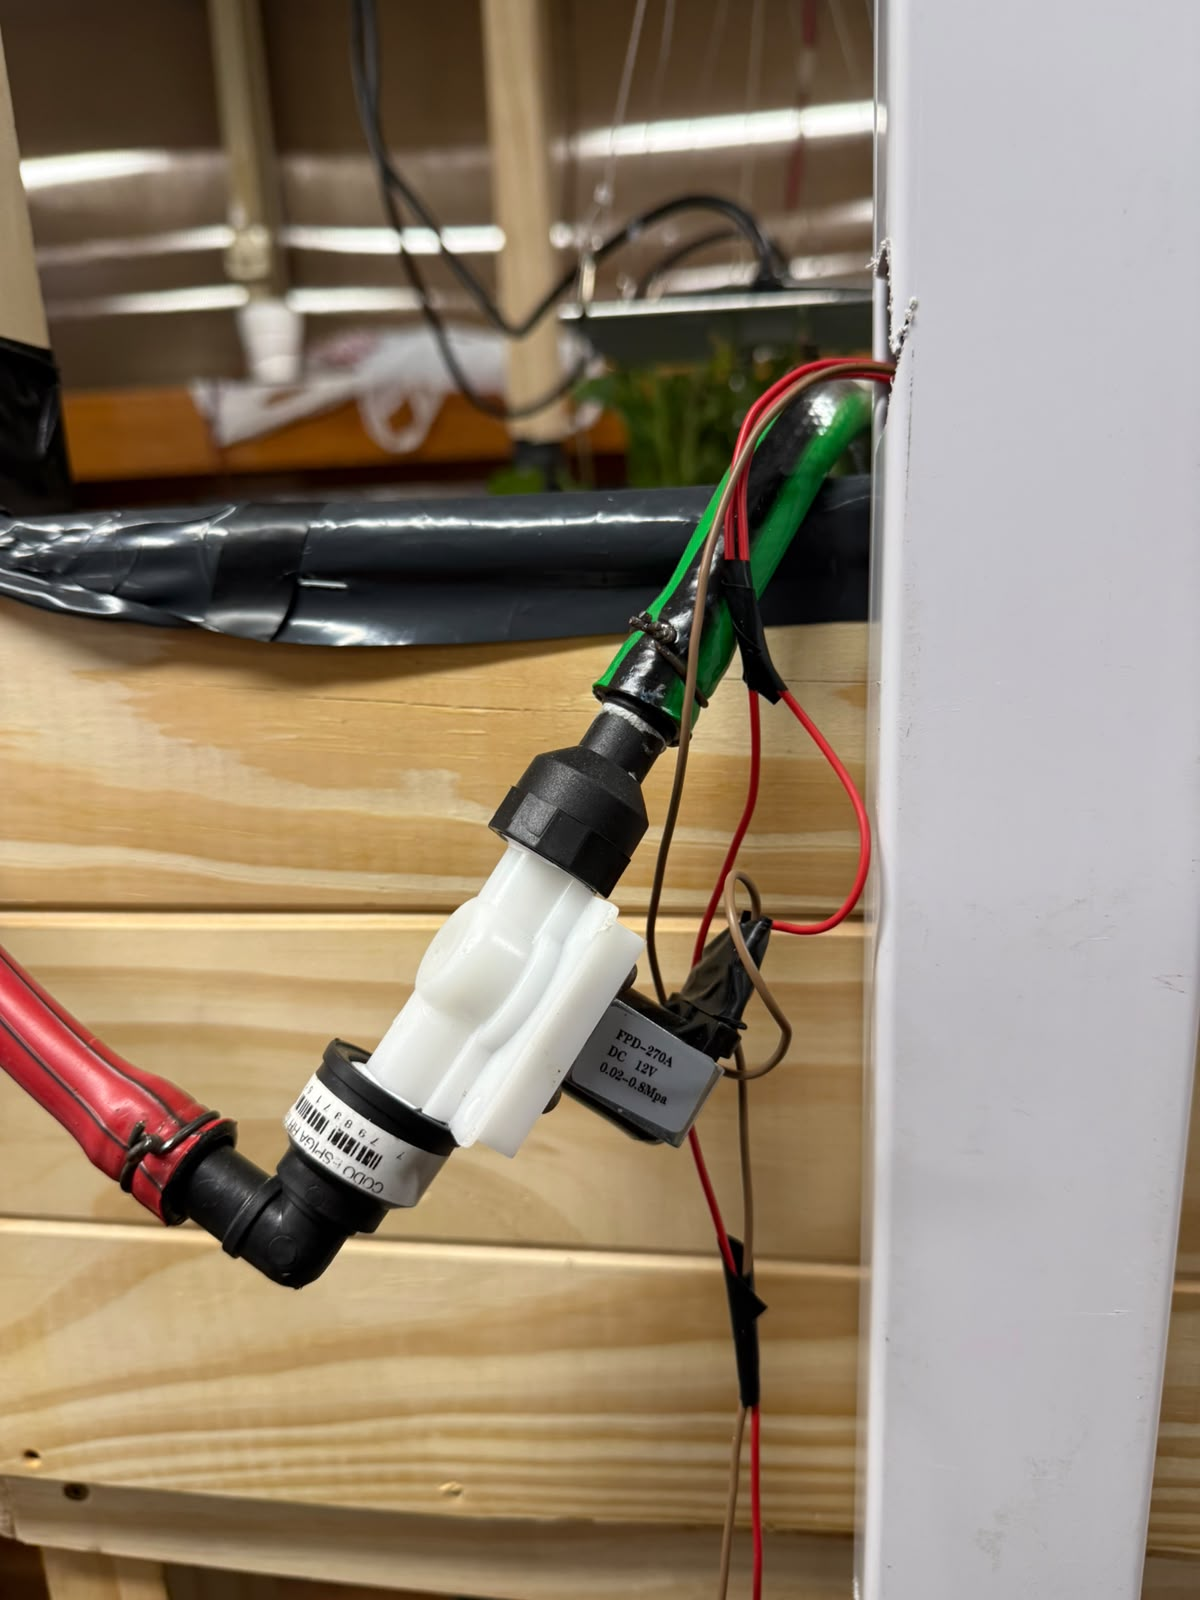
\includegraphics[height=10cm, width=\textwidth, keepaspectratio]{Imagenes/valvsolenoide.jpeg}
    \caption{Valvula solenoide.}
    \Fuente{propia.}
\end{figure}
Una vez que el sustrato absorbe la humedad necesaria para la nutrición y desarrollo vegetal, el excedente no retenido inicia un proceso de percolación natural. Gracias al diseño en pendiente y al sistema de drenaje inferior de cada módulo, el agua no aprovechada cae por acción de la gravedad hacia un depósito de recolección ubicado en la base de la estructura. Este circuito cerrado permite recircular el efluente hídrico hacia el tanque principal mediante una red de colectores, maximizando la eficiencia en el uso del agua y reduciendo de forma significativa el consumo operativo del prototipo.
\begin{figure}[H]
    \centering
    \begin{minipage}{0.48\textwidth}
        \centering
        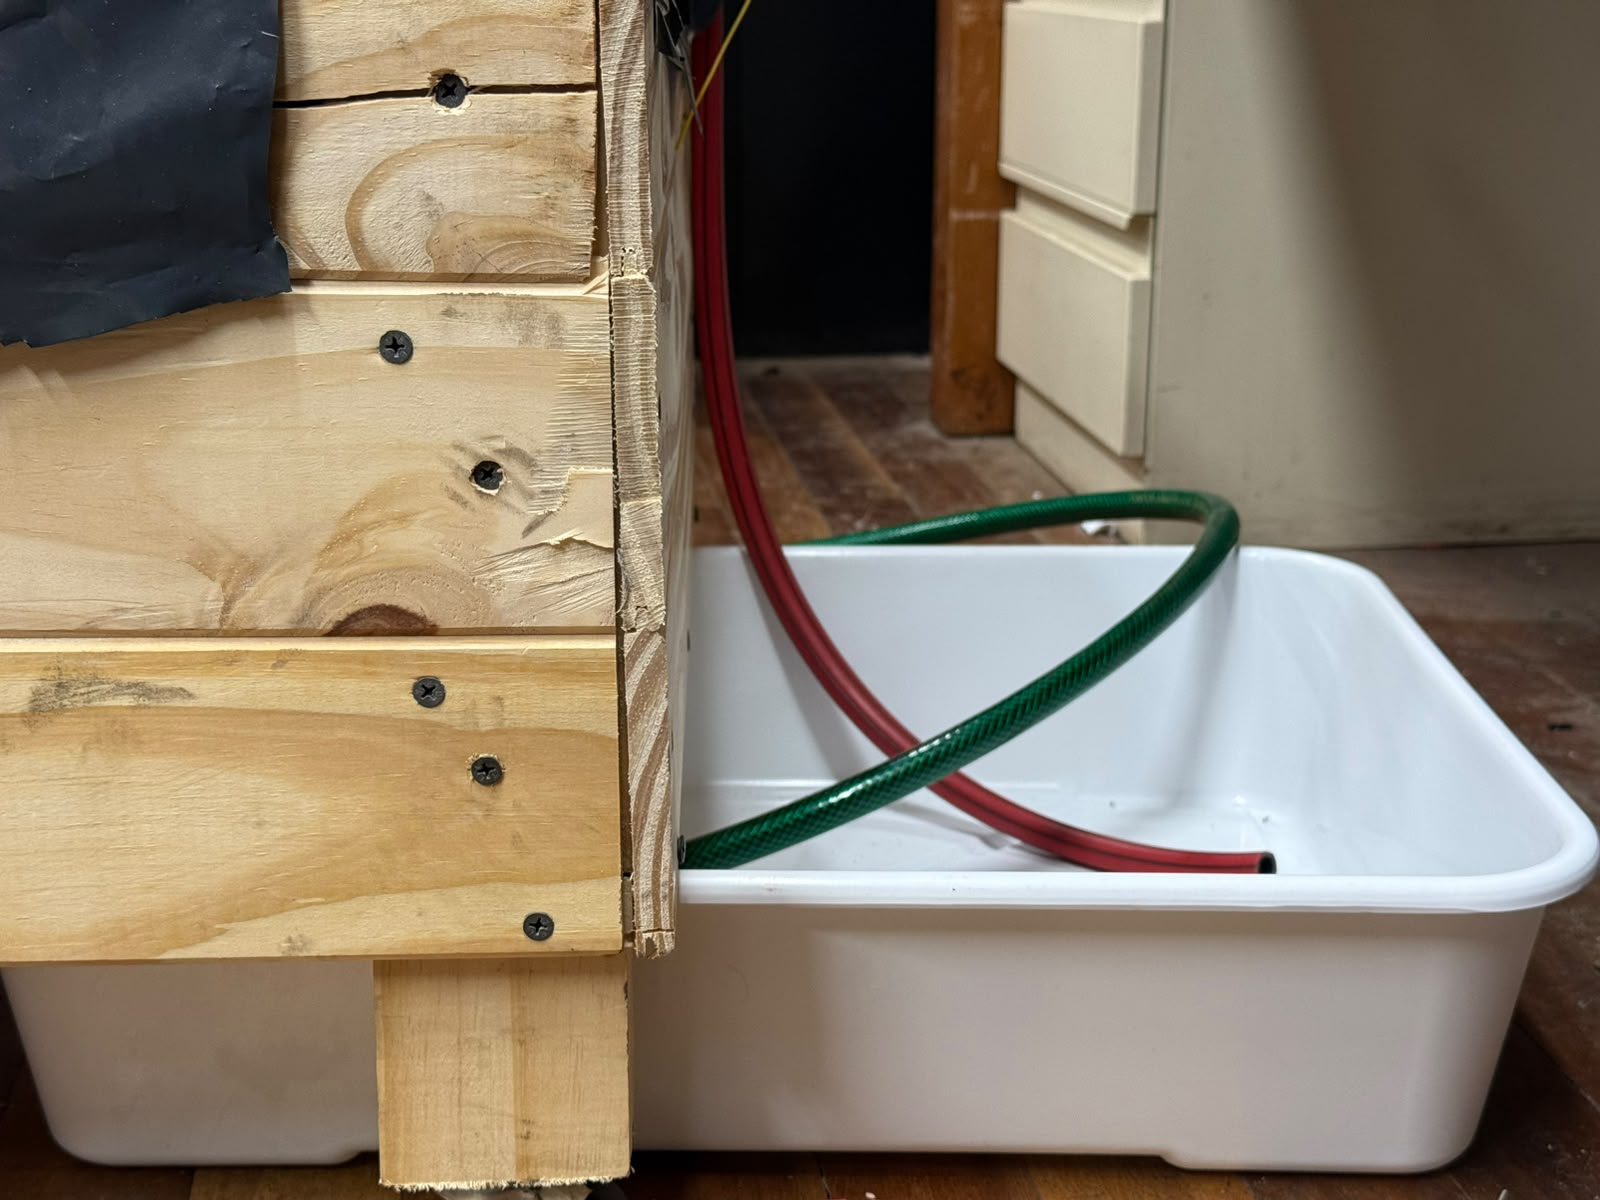
\includegraphics[width=\textwidth]{Imagenes/batea.jpeg}
    \end{minipage}
    \hfill
    \begin{minipage}{0.48\textwidth}
        \centering
        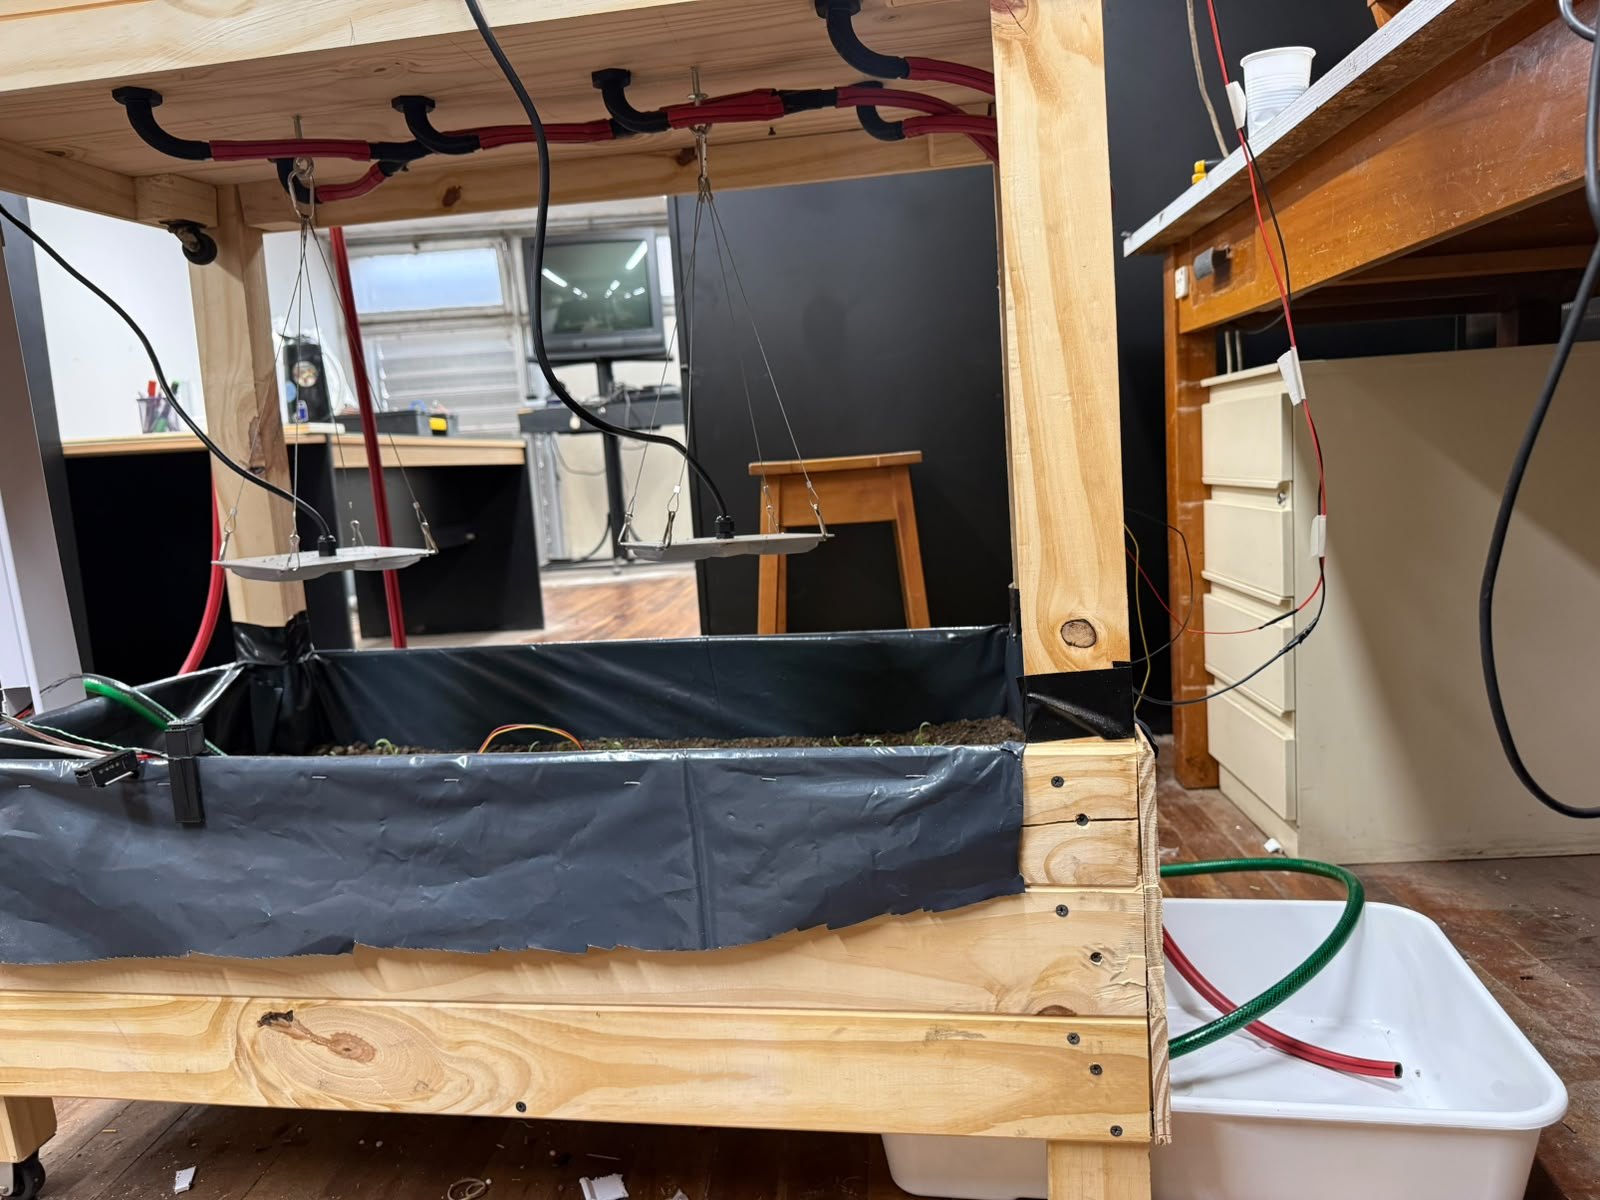
\includegraphics[width=\textwidth]{Imagenes/bateaymaceta.jpeg}
    \end{minipage}
    \caption{Sistema de recolección de agua.}
    \Fuente{propia.}
    \label{fig:soporte_mangueras}
\end{figure}

\section{Sistema de ventilacion}
Con el objetivo de garantizar una renovación constante de la masa de aire y evitar la formación de microclimas saturados de humedad en el dosel vegetal, se integró un sistema de ventilación forzada distribuido por niveles en la estructura vertical. La presencia de humedad relativa elevada y aire estancado favorece la acumulación de condensación sobre el filoplano (superficie foliar), creando un entorno propicio para la proliferación de hongos. Para mitigar este riesgo y favorecer la disipación térmica, se instalaron ventiladores en cada uno de los niveles de cultivo. Estos dispositivos son gestionados dinámicamente por la unidad central mediante un algoritmo de control basado en un umbral crítico de humedad relativa: cuando los sensores del nivel detectan valores superiores al límite configurado, el sistema conmuta la activación de los ventiladores correspondientes. Esta acción rompe la capa límite de humedad sobre las hojas, acelera la tasa de transpiración vegetal de forma controlada y promueve un descenso paulatino de la temperatura ambiental en el módulo.
\begin{figure}[H]
    \centering
    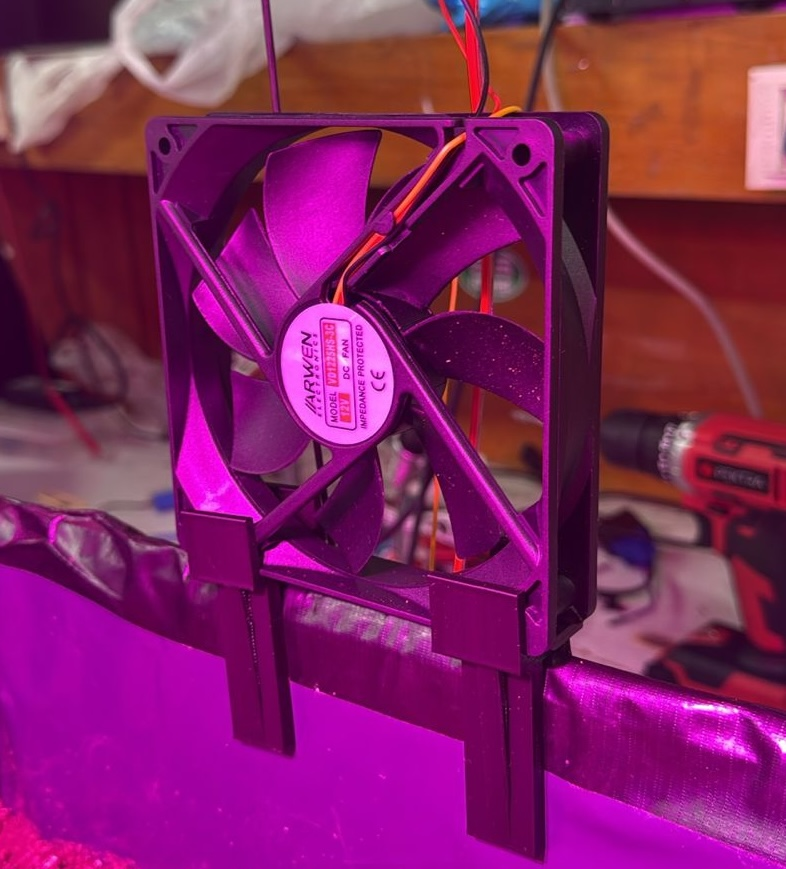
\includegraphics[height=10cm, width=\textwidth, keepaspectratio]{Imagenes/soporteventilador2.jpeg}
    \caption{Disposicion de los ventiladores.}
    \Fuente{propia.}
\end{figure}

\section{Codigo}
hubo que iniciar gpios en 0...

\subsection{Telemetría y Visualización en la Nube: Integración con ThingSpeak}
Para dotar al sistema de capacidades de monitoreo remoto propias del Internet de las Cosas (IoT), se implementó la plataforma en la nube ThingSpeak. Desarrollada por MathWorks, esta herramienta permite la agregación, visualización y análisis de flujos de datos en tiempo real. 

La elección de esta plataforma para el prototipo se fundamenta en múltiples ventajas operativas. En primer lugar, ofrece un nivel de uso gratuito y de libre acceso para proyectos académicos y de investigación, lo que elimina los costos de licenciamiento o alquiler de servidores privados. En segundo lugar, descentraliza la visualización de los datos; al enviar las lecturas críticas del entorno radicular y ambiental a la nube, el usuario adquiere la capacidad de auditar el estado del cultivo (humedad de suelo, iluminancia, temperatura y humedad relativa) desde cualquier dispositivo con acceso a Internet, independizándose de la red de área local donde opera el sistema. Esta arquitectura sienta las bases prácticas para la interconexión de múltiples granjas inteligentes en un futuro.

\subsubsection{Arquitectura de Transmisión de Datos}

El envío de la información hacia los servidores en la nube se ejecuta de manera cíclica en cada iteración del lazo de control principal del sistema. Para garantizar una comunicación eficiente y segura, el algoritmo de telemetría se estructuró en las siguientes etapas conceptuales:

\begin{itemize}
    \item \textbf{Autenticación y Acondicionamiento:} El proceso inicia con la validación de credenciales mediante una clave de interfaz (API Key) única, la cual autoriza a la placa central a publicar información en su respectivo canal. Previo a la conformación del paquete de datos, las lecturas de los sensores sufren un proceso de acondicionamiento digital; los valores decimales son truncados para eliminar fluctuaciones minúsculas no representativas, optimizando así el ancho de banda y el peso de la trama de red enviada.
    
    \item \textbf{Tolerancia a Fallos y Operación Local:} El aspecto más crítico de la rutina de transmisión es su diseño orientado a la robustez. La comunicación con los servidores externos incorpora mecanismos de seguridad como la limitación del tiempo máximo de espera (\textit{timeout}) y el manejo seguro de excepciones ante caídas de conexión. 
    
    \item \textbf{Prioridad de Control:} Estas medidas garantizan que, ante una eventual pérdida de acceso a Internet o latencia en los servidores remotos, el software no colapse ni detenga su ejecución. De este modo, la unidad central prioriza el control local, pudiendo continuar ininterrumpidamente con tareas críticas como la desactivación de la bomba de riego o el encendido de la iluminación, asegurando la integridad del cultivo sin importar el estado de las telecomunicaciones.
\end{itemize}

agregar fotos

\section{UI: Interfaz de Usuario}

agregar fotos

\section{Esquemas de conexion}
A continuación, se detalla el esquema de conexionado adoptado para el prototipo, describiendo la asignación de señales para cada puerto de propósito general de la unidad central. Por criterios de diseño orientados a la robustez electromecánica, se proyectó una interfaz intermedia mediante una placa de circuito impreso perforada de uso general, la cual actúa como un nodo centralizador de conexiones. Esta implementación previene la necesidad de efectuar uniones soldadas directas sobre la computadora de placa única, resguardando la integridad física de sus terminales y flexibilizando la modularidad del sistema ante tareas de mantenimiento o sustitución de periféricos. En el diagrama esquemático, la denominación de "Componentes i2c" identifica el nodo de acoplamiento para el bus de datos compartido, donde coexisten bajo el mismo direccionamiento el sensor de iluminancia y el módulo de conversión analógico digital, el cual gestiona de forma dedicada los canales de los higrómetros capacitivos de suelo.
\begin{figure}[H]
    \centering
    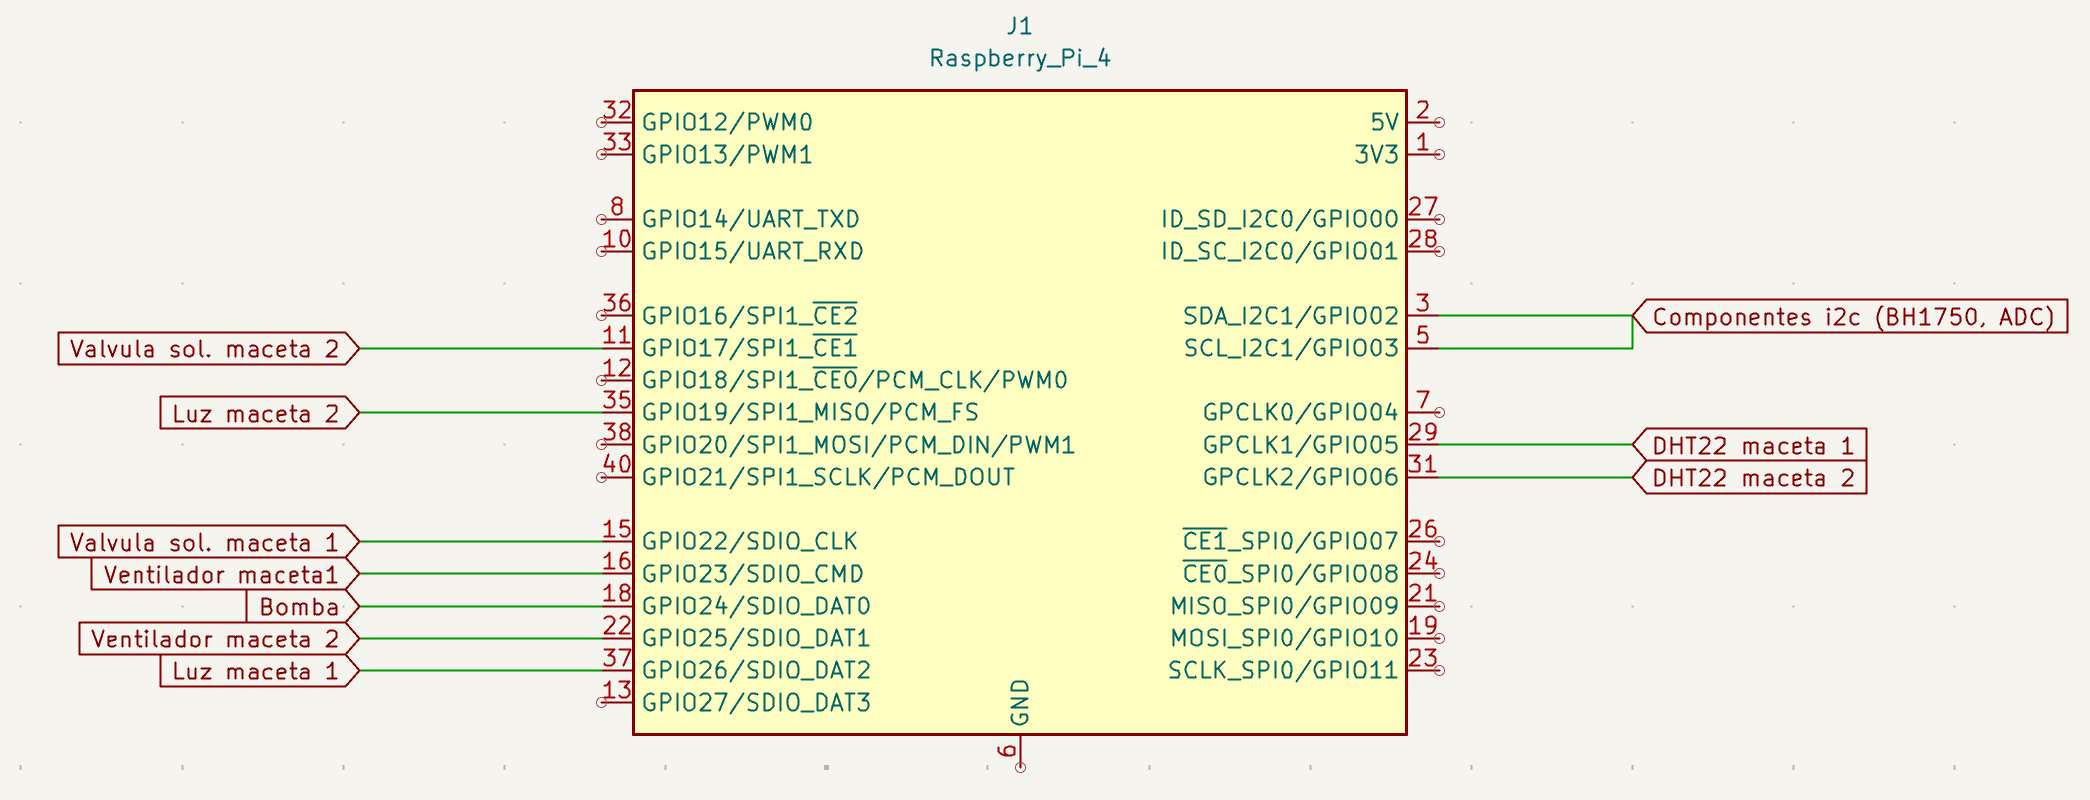
\includegraphics[height=10cm, width=\textwidth, keepaspectratio]{Imagenes/RaspberryPi4Schematic.png}
    \caption{Esquema de conexiones.}
    \Fuente{propia.}
\end{figure}
\begin{figure}[H]
    \centering
    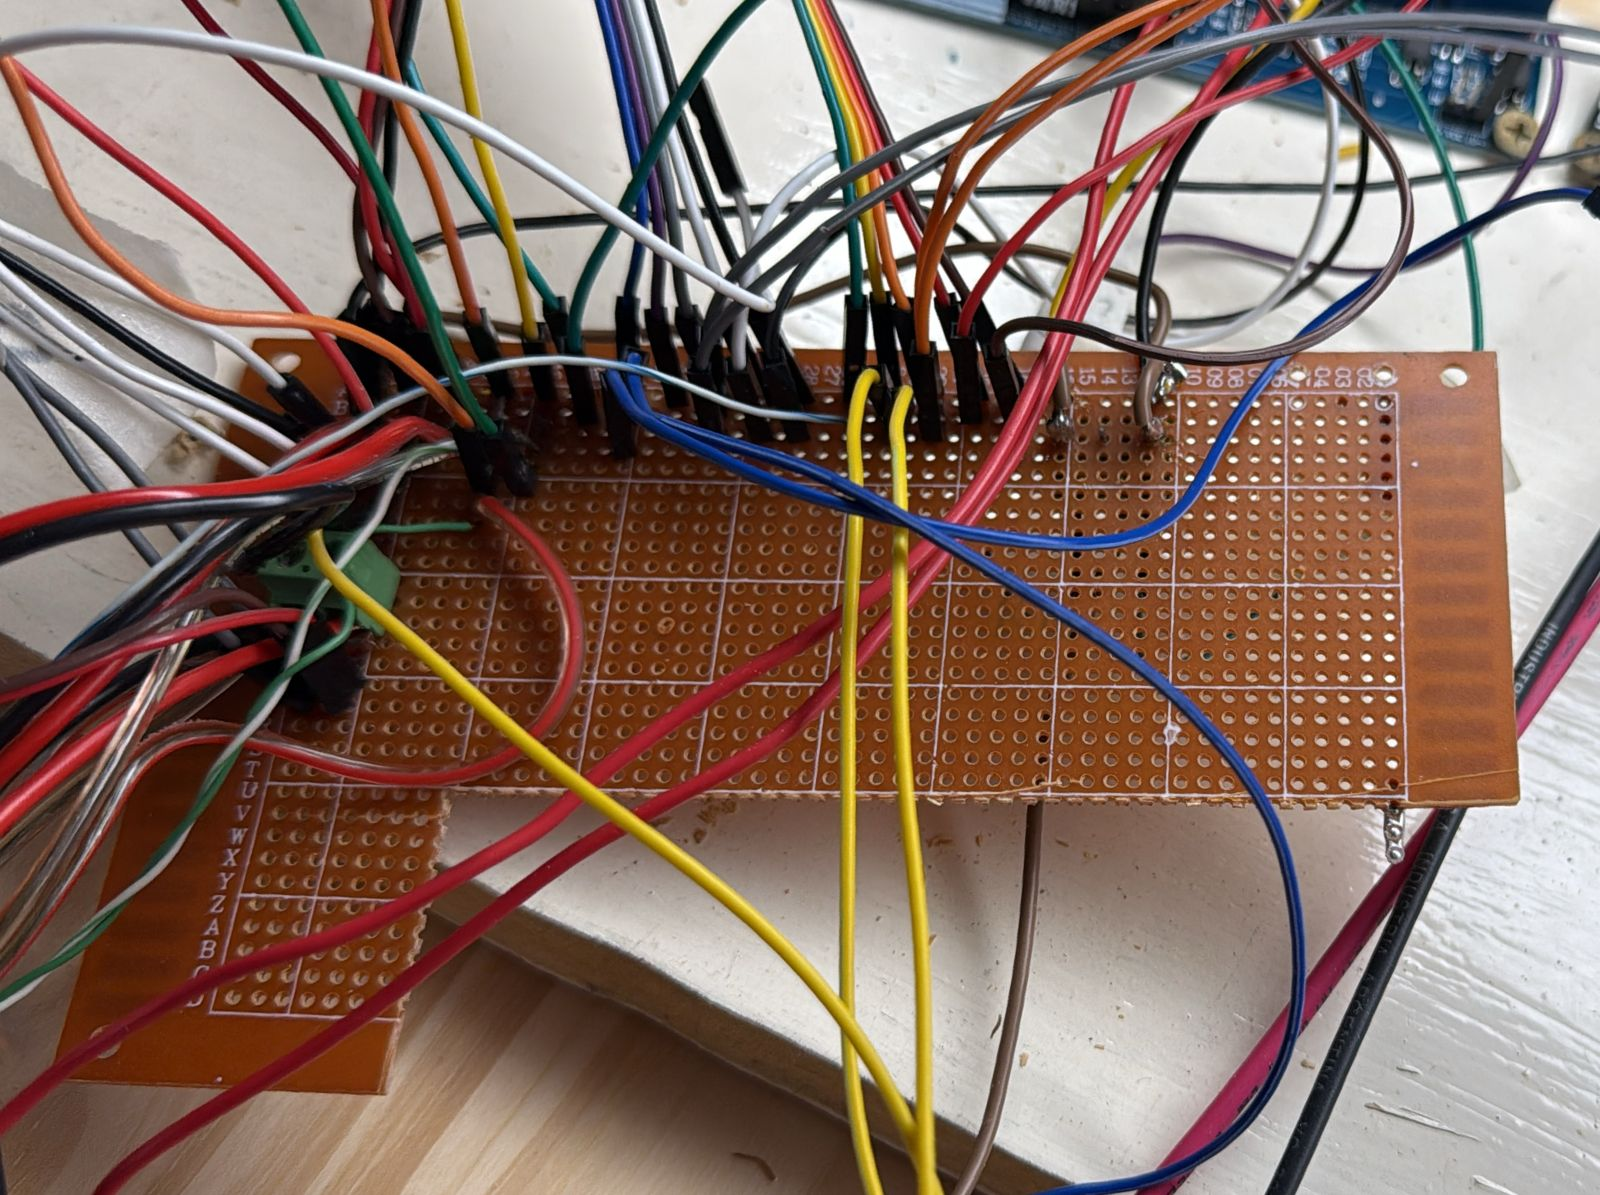
\includegraphics[height=10cm, width=\textwidth, keepaspectratio]{Imagenes/placaperforada.jpeg}
    \caption{Placa perforada de uso general.}
    \Fuente{propia.}
\end{figure}
Diagrama de conexion de la placa mostrada en la imagen anterior:
\begin{figure}[H]
    \centering
    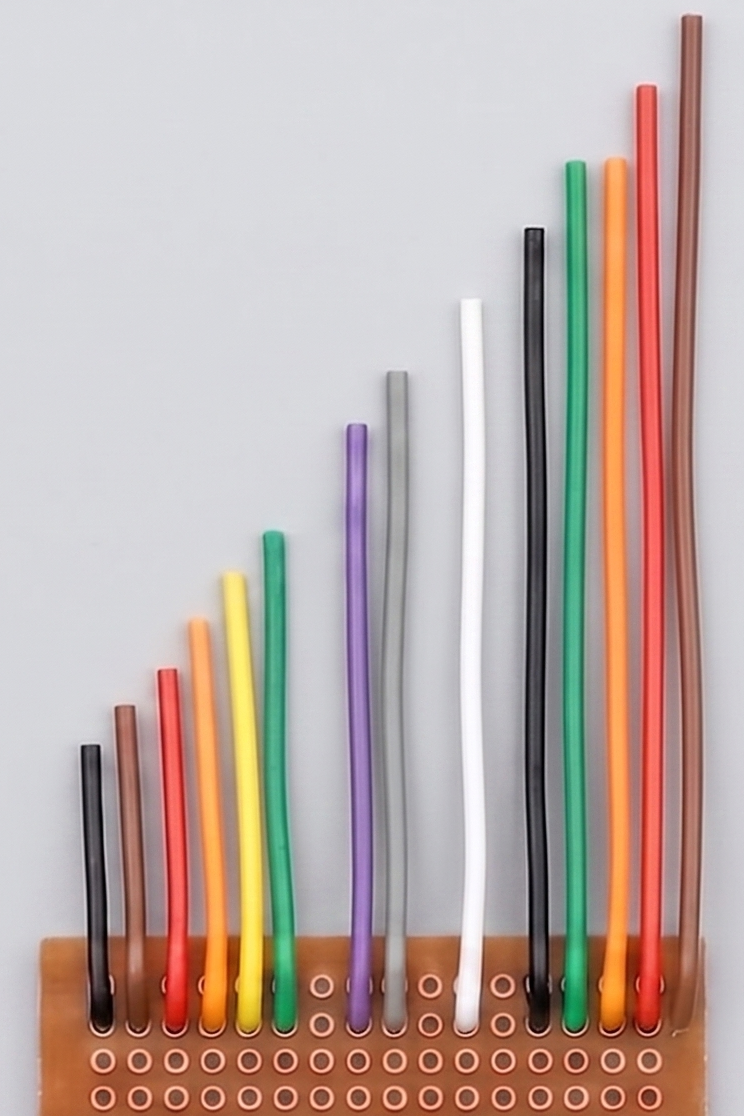
\includegraphics[height=10cm, width=\textwidth, keepaspectratio]{Imagenes/ProtoCables1.png}
    \caption{Esquema de placa de pruebas simplificado con color de cables.}
    \Fuente{propia.}
\end{figure}
\begin{figure}[H]
    \centering
    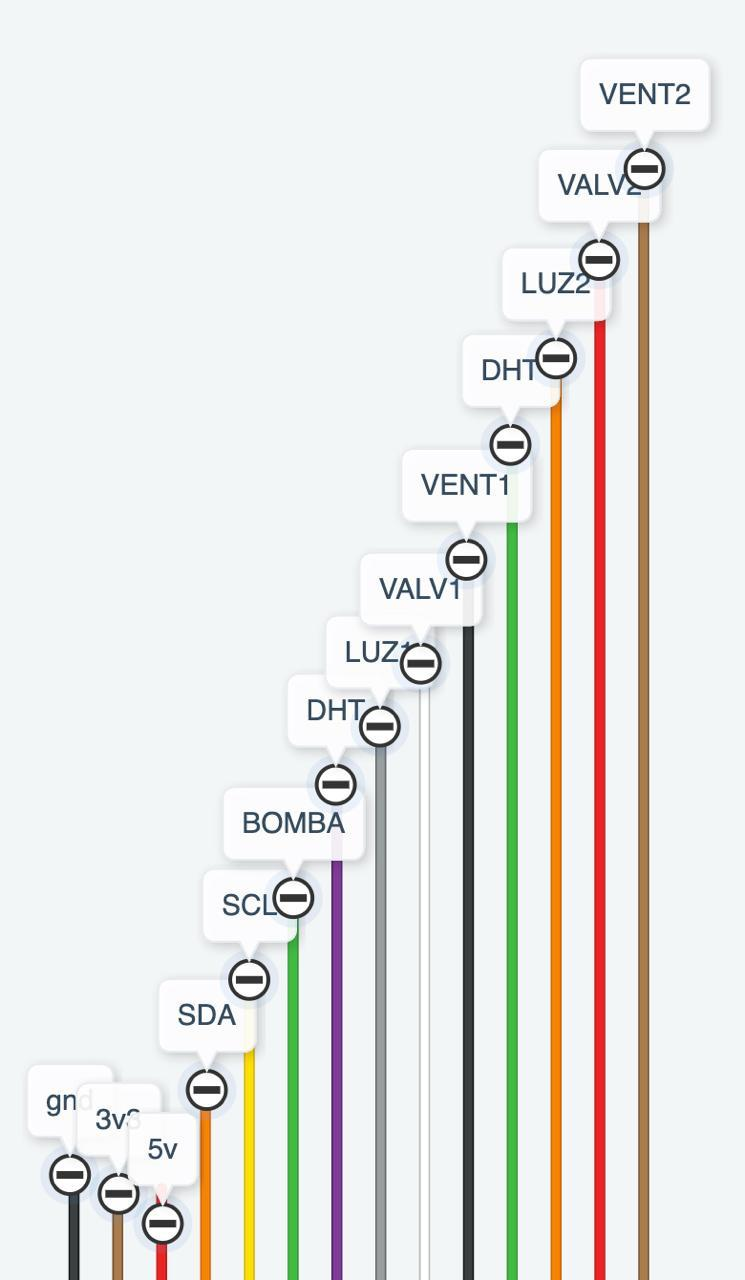
\includegraphics[height=10cm, width=\textwidth, keepaspectratio]{Imagenes/protocables2.jpeg}
    \caption{Conexion que recibe cada color de cable en relacion al esquema anterior.}
    \Fuente{propia.}
\end{figure}

\section{Consumo de potencia}
Con el propósito de auditar la demanda energética máxima del prototipo y validar el correcto dimensionamiento de las etapas de alimentación, se llevó a cabo una prueba de caracterización bajo el régimen de operación a plena carga. Este ensayo consistió en la activación simultánea y continuada de la totalidad de los actuadores de potencia, incluyendo los paneles lumínicos, la electrobomba hidráulica, la red de ventilación forzada y la unidad central de procesamiento en estado de cómputo activo junto a la matriz de sensado. Mediante la inserción de una pinza amperimétrica en la línea principal de suministro, se registró el consumo de corriente pico instantáneo y en régimen permanente. La Figura descrita a continuación ilustra el procedimiento instrumental de medición, cuyo valor obtenido permite determinar la potencia activa total consumida por la granja inteligente en su punto de máxima exigencia operativa y verificar los márgenes de seguridad térmica en los conductores.
\begin{figure}[H]
    \centering
    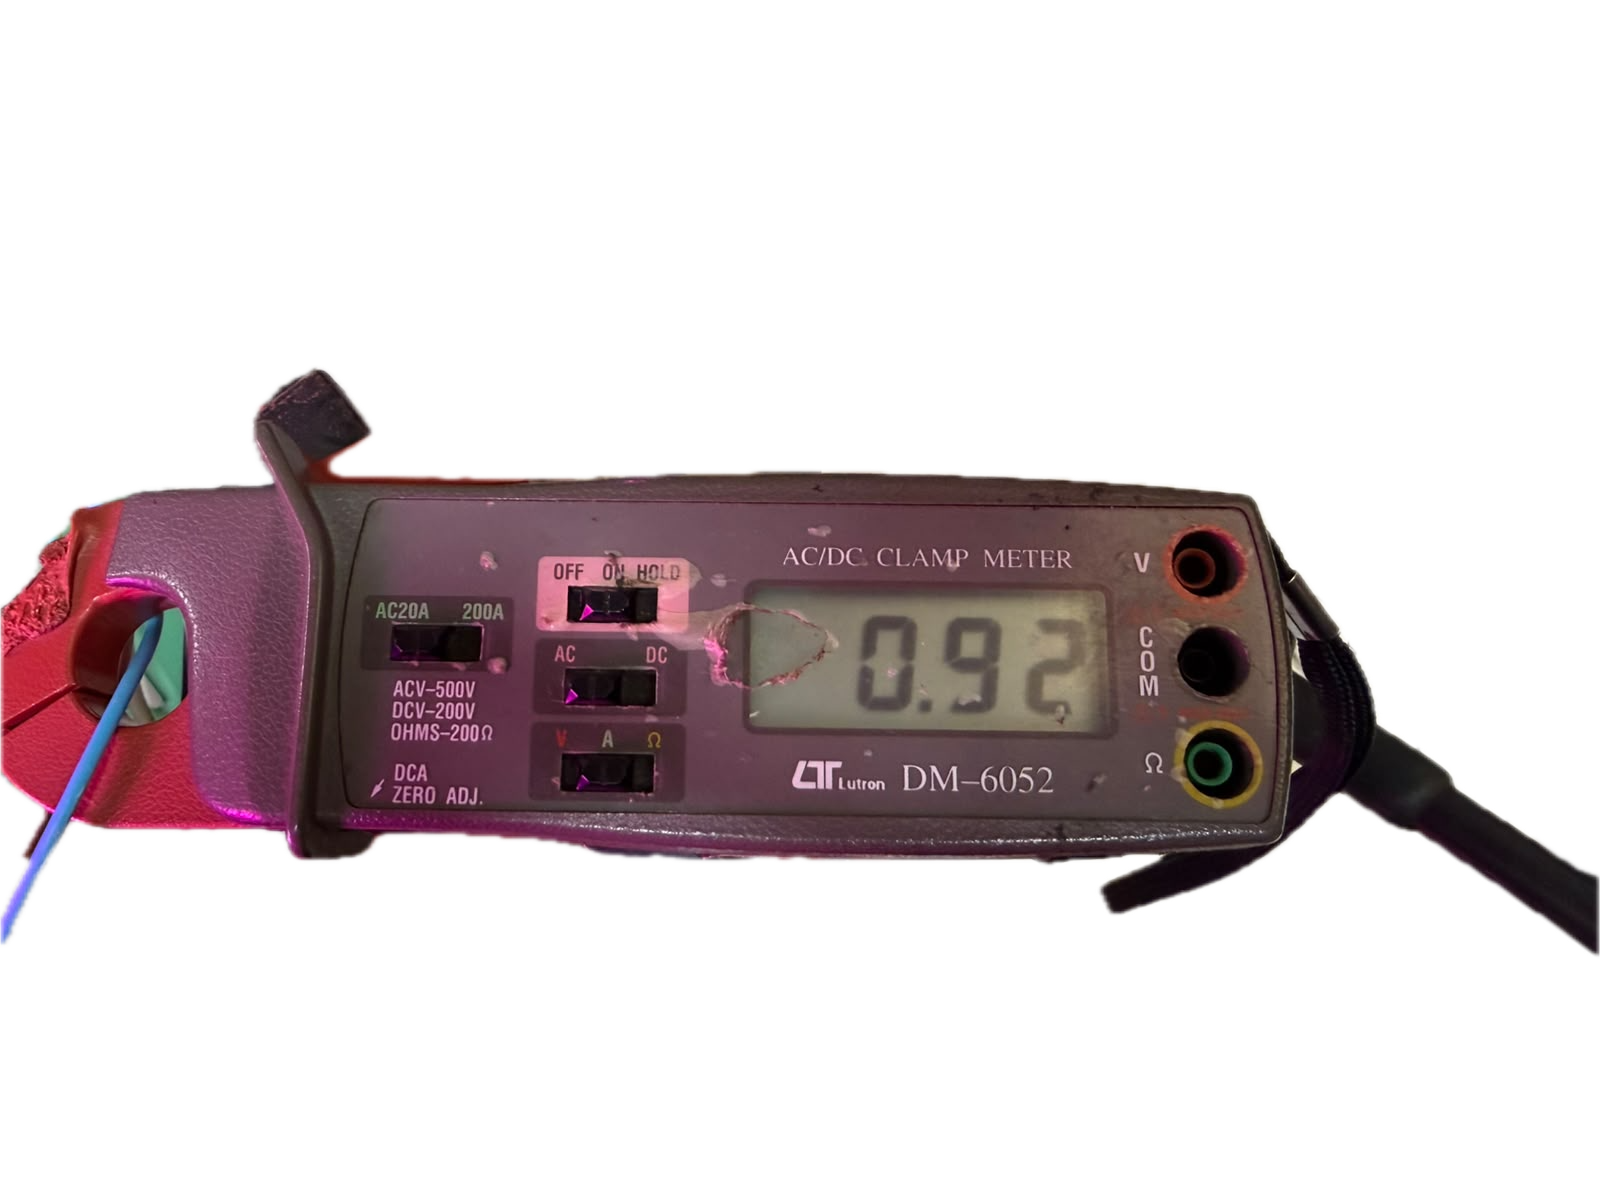
\includegraphics[height=10cm, width=\textwidth, keepaspectratio]{Imagenes/consumo.png}
    \caption{Lectura del amperimetro en [A].}
    \Fuente{propia.}
\end{figure}
A continuacion calculamos la potencia instantanea [W] consumida por el prototipo:
\begin{align}
    P &= V \cdot I \nonumber \\
    P &= 220\text{ V} \cdot 0{,}92\text{ A} \nonumber \\
    P &= 202{,}4\text{ W} \label{eq:desarrollo_potencia}
\end{align}
Luego, el calculo del consumo de potencia por hora [kWh] es:
\begin{align}
    P &= \frac{P \cdot t}{1000}\nonumber \\
    P &= \frac{202,4W \cdot 1hs}{1000}\nonumber \\
    P &= 0,202kWh \label{eq:calculo_kwh}
\end{align}

Desde la perspectiva electro-energética, el prototipo demostró un nivel de eficiencia que valida su implementación técnica en entornos urbanos y residenciales. El consumo máximo registrado a plena carga (donde ocurre la activación simultánea de los paneles LED, la electrobomba, las válvulas solenoides, la ventilación forzada y el procesamiento continuo de la Raspberry Pi 4b) se estabilizó en $202{,}4\text{ W}$. Este valor nominal resulta sumamente acotado, siendo equivalente a la demanda de un equipo informático de escritorio estándar. 

Es fundamental destacar que este consumo pico no representa la demanda sostenida del sistema. Gracias a la arquitectura de control implementada en la unidad central, los actuadores operan bajo ciclos de trabajo (\textit{duty cycles}) estrictamente optimizados. Mientras que la instrumentación lógica (Raspberry Pi y red de sensores) requiere alimentación ininterrumpida con un impacto energético marginal, las cargas de mayor potencia se gestionan de forma intermitente: el fotoperíodo de las luminarias limita su uso a una fracción del día, y la bomba junto con las válvulas solenoides se activan únicamente durante las breves ventanas de irrigación. 

En conclusión, el balance energético del sistema confirma la viabilidad económica y ambiental del cultivo automatizado indoor. El diseño de hardware seleccionado permite mantener un ecosistema biológico complejo sin sobrecargar la infraestructura eléctrica domiciliaria, sentando las bases para escalar el proyecto añadiendo nuevos módulos de cultivo con un impacto energético predecible y sostenible.

